%=-=-=-=-=-=-=-=-=-=-=-=-=-=-=-=-=-=-=-=-=-=-=-=-=-=-=-=-=-=-=-=-=-=-=-=-=-=-=-=-=-=-=-=-=-=
% Preamble - Cal Poly Thesis Based on UC Thesis Format
%=-=-=-=-=-=-=-=-=-=-=-=-=-=-=-=-=-=-=-=-=-=-=-=-=-=-=-=-=-=-=-=-=-=-=-=-=-=-=-=-=-=-=-=-=-=
\documentclass[12pt]{ucthesis}
\usepackage{thesis_preamble}
\usepackage{cmap}
\usepackage{verbatim}
\usepackage{listings}
\usepackage{float}
\usepackage{titlesec}
\usepackage{nomencl}
\usepackage{multicol}
\widowpenalty 10000
\clubpenalty 10000

\title{FLIGHT TESTING SMALL UAVS FOR AERODYNAMIC PARAMETER ESTIMATION}
\author{Adam T. Chase}
\degreemonth{February} \degreeyear{2014} \degree{Master of Science}
\defensemonth{February} \defenseyear{2014}
\numberofmembers{4} \chair{Robert McDonald, Ph.D.} \othermemberA{Eric Mehiel, Ph.D.} \othermemberB{Russell Westphal, Ph.D.} \othermemberC{Kurt Colvin, Ph.D.}
\field{Aerospace Engineering} \campus{San Luis Obispo} \copyrightyears{seven}

%=-=-=-=-=-=-=-=-=-=-=-=-=-=-=-=-=-=-=-=-=-=-=-=-=-=-=-=-=-=-=-=-=-=-=-=-=-=-=-=-=-=-=-=-=-=
% Document
%=-=-=-=-=-=-=-=-=-=-=-=-=-=-=-=-=-=-=-=-=-=-=-=-=-=-=-=-=-=-=-=-=-=-=-=-=-=-=-=-=-=-=-=-=-=
\makeatletter

\def\@makechapterhead#1{%
  \vspace*{2\p@}%
  {\parindent \z@ \raggedright \normalfont
    \ifnum \c@secnumdepth >\m@ne
        \normalfont\normalsize\bfseries \thechapter
.0~ %NOTE: this is supes jenky. might give problems later.
    \fi
    \interlinepenalty\@M
    \normalsize \bfseries #1\par\nobreak
    \vskip 1\p@
  }}
  \makeatother
  
  %redefine cite to be a superscript
  \let\oldcite\cite
  \renewcommand{\cite}[1]{\textsuperscript{\oldcite{#1}}}
  
\renewcommand*\nompreamble{\begin{multicols}{2}}
\renewcommand*\nompostamble{\end{multicols}}

\begin{document}

\maketitle

\begin{frontmatter}
	
	\copyrightpage
	%\approvalpage
	\committeemembershippage

	\pdfbookmark[0]{Abstract}{abs} % Sets a PDF bookmark for the abstract
\begin{abstract}
%todo:I think this is fine
\begin{abstract}
A flight data acquisition system was developed to aid unmanned vehicle designers in verifying the system's design performance. The system is reconfigurable and allows the designer to choose the correct combination of complexity, risk, and cost for a given flight test, as well as allowing the designer to reconfigure the system to meet packaging requirements. System functionality was validated by collecting data during flight of an radio-controlled aircraft, and future work includes further system validation, quantifying system accuracy, sensor fusion, and stability and control derivative estimation.
\nomenclature{UAS}{Unmanned aerial system}
\nomenclature{R/C}{Radio-controlled}
\end{abstract}
\end{abstract}

\begin{acknowledgements}
I'd first like to thank my friends and fellow Flight Lab people. Each of you brought something good to my time at Poly. B$^2$ and Cory, you guys were awesome roommates and made the Stafford house fun. Alex, Brian, Christian, Trevor, Mike, and the rest of the DBF/Flight Lab crew, you guys made that window-less lab bearable, and occasionally downright enjoyable. \#W9W

I'd also like to thank my committee. Throughout my Cal Poly career every member of the committee has helped me immensely. Dr. Colvin, hosting Akaflieg barbecues at your hangar introduced my to a side of aviation I hadn't seen, and gave me passion for aircraft and flight. Dr. Mehiel, you've provided countless guidance throughout school, ranging from classes and scheduling to Lyapunov stability and Kalman filters. Dr. Westphal, the Edward's project was a great experience for me, and you've been incredibly supportive with anything and everything I've needed help with since. And Dr. McDonald, you've given me countless opportunities, including DBF, Edwards, LENR, Senior Design, R/MAX, this thesis, ... For five and a half years, you've guided me through challenging problems, taught me to think like an engineer, and ignored DBF t-shirts and team names. Thank you, it's been a pleasure.

Finally, my family. The entire family (aunts, uncles, grandparents, etc.) have supported me the whole way through, and I'm very grateful for that. I can't put into words the opportunities and support my parents and sister have given me. Mom, Dad, Jackie: Thank you. You guys are awesome.
\end{acknowledgements}


\addcontentsline{toc}{chapter}{TABLE OF CONTENTS}
\tableofcontents


\listoftables

\listoffigures

\printnomenclature

\end{frontmatter}

\pagestyle{plain}

\renewcommand{\baselinestretch}{1.66}



% ------------- Main chapters here --------------------
%todo:i think this is fine
\chapter{Introduction}
\label{intro}
Aircraft designers often use model fits and ``rules of thumb'' to successfully complete designs, with many of these guidelines available in various design textbooks. \cite{raymer}$^,$\cite{nicolai2010fundamentals}$^,$\cite{roskam1985airplane} These models and practices have been established based on years of data analysis and validation that the designs perform as expected. However, the scope of these empirical design techniques is limited to the input of the regression model: an intelligent designer will not use a general aviation weight model for a transport category aircraft. To this end, there is a significant lack of small UAV-class guidelines for designing an aircraft.

 Accurate estimations of a small-scale vehicle's lift and drag characteristics are extremely critical to the aircraft designer, and affect both point performance (turn rates, climb rates, stall speeds, etc.) and mission performance (range and endurance). Much of the prediction tools available in the classic lift and drag textbooks from Hoerner\cite{hoernerDrag}$^,$\cite{hoernerLift} only apply to larger scale structures. In addition, drag prediction is extremely difficult on small vehicles, as some sources of drag are not easily modeled. For instance, actuator control horns and protruding screw heads are not typically included in the CFD \nomenclature{CFD}{Computational fluid dynamics} analysis of aircraft. However, for small vehicles, these sources of ``crud'' drag can be a significant portion of the total vehicle's drag value. 
 
 One advantage of small UAVs is that they are fairly inexpensive, which makes building multiple fully-functioning prototypes a viable option. The authors chose to take advantage of this fact and develop a flight data acquisition system with a primary goal of measuring the lift and drag characteristics of a small UAV. This would enable vehicle designers to build a conceptual-design-level prototype, and both develop and validate predictive, regression-based models. The system would also allow designers to conduct quantitative trade studies, such as the trade between drag reduction technologies (wheel pants, retractable landing gear, winglets, etc.) and the weight associated with them.\\

The authors also desired additional sensors to aid designers with more than just lift and drag characteristics. Some areas of interest are estimating stability and control derivatives, as well as possible control algorithm testing, in-flight thrust measurement, and payload integration capabilities. To accomplish these goals, sensors not directly necessary to lift and drag estimation were included in the overall system. The system was also designed in a manner that made it reconfigurable. This allows future designers to decide what combination of accuracy, risk, and sensing capabilities they need on a given flight test, and to then package the sensors in a manner that meets vehicle integration requirements.\\

For this paper, the authors chose to integrate the necessary sensors to estimate lift and drag forces, as well as those necessary for a basic INS\nomenclature{INS}{Inertial navigation system}, ambient temperature measurement, and servo and motor signals. The system will be validated by measuring the as-built drag polar of an R/C aircraft, as well as all other available states the system is capable of measuring.
%todo: add back in derivation of "drag polar"? Remove kalman filter section. Method section should be alright.
\chapter{Method}
\label{background-information}
Some basic assumptions will apply throughout the modeling of dynamics in this paper. They are as follows:
\begin{enumerate}
\item The vehicle is a fixed mass.
\item Coriolis effects are negligible.
\item Thrust will be assumed to be 0.
\end{enumerate}
Note that a stationary atmosphere is not assumed. The fixed mass assumption is consistent with the electric aircraft used to test the system. At the altitude and speed at which the vehicles will be tested, Coriolis effects can be ignored\cite{klein2006aircraft}. The zero-thrust assumption is in place to minimize drag error. Any error in a measured state will decrease the accuracy of the drag measurement, and the accuracy of a given drag measurement can be no better than the worst state measurement error. In-flight thrust is difficult to measure accurately, so a folding propeller will be used, and the motor will be turned off during data acquisition. This will allow the propeller to fold back, eliminating most of the wind-mill drag associated with a stalled propeller. 

\section{Reference Frames}
The reference frames used in this paper will follow standard convention\cite{klein2006aircraft}, but will be repeated for clarity. The NED frame is a vehicle carried frame, with the $+\hat{i}$ axis pointing due North, the $+\hat{j}$ axis pointing due East, and the $+\hat{k}$ axis pointing toward the center of the earth. The body axis system, defined by the body-mounted accelerometer, is a right handed coordinate system, with the $+\hat{i}$ axis pointing out the nose of the aircraft, the $+\hat{j}$ axis pointing out the right wing, and the $+\hat{k}$ axis pointing out the bottom of the vehicle. The wind axes are a vehicle-carried coordinate system, with the origin at the same location as the body reference frame. The $\hat{i}$ axis of the wind reference frame points in the direction of the free-stream velocity. The $\hat{k}$ direction lies in the x-z plane of the body reference frame. The $\hat{j}$ direction is then defined to be out the right side of the vehicle, in order to follow the right hand rule. 

\section{Equations of Motion}
\label{sys-desc}
Newton's 2nd Law of Motion states
\begin{align}
\Sigma\vec{F} &= \frac{d}{dt}(\vec{mV})
\end{align}
\noindent
where $\Sigma\vec{F}$ is the sum of all applied forces, $\vec{m}$ is the mass of the vehicle, and $\vec{V}$ is the vehicle's velocity. Using the fixed mass assumption, this reduces to 
\begin{align}
\Sigma\vec{F} &= m\frac{d\vec{V}}{dt}\\
&= m\vec{a}
\end{align}

The applied forces on the vehicle for drag polar estimation are 
\begin{align}
\Sigma\vec{F} &= \vec{F}_{A}+\vec{F}_{G}+\vec{F}_{T}
\end{align}
\nomenclature{$\vec{F}_A$}{Aerodynamic forces}
\nomenclature{$\vec{F}_G$}{Gravitational forces}
\noindent
where $\vec{F_{A}}$ accounts for all aerodynamic forces acting on the vehicle, $\vec{F_{G}}$ is the force due to gravity, and $\vec{F_{T}}$ accounts for forces from the propulsion system, which are assumed to be zero.\\
Aerodynamic forces can be described in the wind reference frame. In general, they are defined as

\begin{align}
\vec{F}_{A_w} &= D \hat{i}_w+Y \hat{j}_w+L \hat{k}_w
\end{align}
\noindent
where $D$ is drag force, $Y$ is side force, and $L$ is lift force.\\
The gravitational force on the vehicle acts in the $+z_{NED}$ direction and is equal in magnitude to the vehicle's weight $W$, leading to
\begin{align}
\vec{F}_{G_{NED}} &= 0\hat{i}_{NED}+0\hat{j}_{NED}+W\hat{k}_{NED}
\end{align}
\nomenclature{NED}{North east down frame}
The aerodynamic and gravity forces can be combined and expressed in the body frame

\begin{align}
m\vec{a}_b &= \vec{F}_{G_b} + \vec{F}_{A_b}
\end{align}
\noindent
which can then be expressed as 
\begin{align}
m\vec{a}_b - m\vec{g} &= \vec{F}_{A_b}\\
m(\vec{a}_b - \vec{g}) &= \vec{F}_{A_b}
\label{accelerometerEqn}
\end{align}

Then, it is noted that a body mounted accelerometer will not measure $\vec{a}_b$, but will instead measure the quantity $\vec{a}_b - \vec{g}$. This means Equation \ref{accelerometerEqn} is really

\begin{align}
\label{plantEqn1}
\vec{F}_{A_b} &= -m\vec{r}_b
\end{align}
where $\vec{r}_b$ is the reading from a body mounted accelerometer. The aerodynamic forces in wind axes, which is the goal, can then be calculated using a rotation matrix
\begin{align}
\label{plantEqn2}
\vec{F}_{A_w} &= \bar{R}^b_w\vec{F}_{A_b}
\end{align}
\nomenclature{$\bar{R}^m_n$}{Rotation matrix from m to n}
Equations \ref{plantEqn1} and \ref{plantEqn2} are important, and show that the only sensors necessary for drag polar estimation during gliding flight are a body-mounted accelerometer and an air data system.

\section{Kalman Filter Usage}
\label{kalman-filter}
This paper utilizes multiple Kalman filters to estimate both regression coefficients and improved states. As a brief overview, the Kalman filter combines the measured state with a predicted state to give an optimal\cite{kalman60} estimate of the actual system state.

\subsection*{Linear Kalman Filter}
A linear Kalman filter can be applied\cite{welch1995introduction} where the system in question can be described in the form 

\begin{align}
x_k &= \bar{A}x_{k-1} + \bar{B}u_{k-1}+w_{k-1}
\end{align}
\noindent
where $\bar{A}$ is the state transition matrix, $x_{k-1}$ is the previous state, $\bar{B}$ is the input matrix, $u_{k-1}$ is the input vector, and $w_{k-1}$ is random process noise.

The measured state is then 
\begin{align}
z_k &= \bar{H}x_k+v_k
\end{align} 
\noindent
where $\bar{H}$ is the output matrix and $v_k$ is measurement noise.\\
The Kalman filter operates in a predictor-corrector manner, where the predictor step is often called the \textit{a priori} estimate, and the corrector step is often called the \textit{a posteriori} estimate. The \textit{a priori} state estimate is calculated using prior states and inputs, while assuming no process noise

\begin{align}
\hat{x}^-_k &= \bar{A}\hat{x}_{k-1}+\bar{B}u_{k-1}
\end{align}

The \textit{a priori} estimate of the covariance matrix is projected in a similar manner

\begin{align}
\bar{P}^-_k &= \bar{A}\bar{P}_{k-1}\bar{A}^T+\bar{Q}
\end{align}
\noindent
where $\bar{P}$ is the covariance matrix and $\bar{Q}$ is the process noise matrix.

The Kalman gain is calculated by combining the predicted, \textit{a priori} covariance matrix with the measurement noise covariance matrix $\bar{R}$

\begin{align}
\bar{K}_k &=\bar{P}^-_k\bar{H}^T(\bar{H}\bar{P}^-_k\bar{H}^T + \bar{R})^{-1}
\end{align}

This optimal Kalman gain is then used to estimate the \textit{a posteriori} estimate of the state and covariance matrix

\begin{align}
\label{kalmanStateUpdate}
\hat{x}_k &=\hat{x}^-_k+\bar{K}_k(z_k-y_k)
\end{align}

\begin{align}
\bar{P}_k &= (\bar{I}-\bar{K}_k\bar{H})\bar{P}^-_k
\end{align}
\noindent
where $y_k$ is the predicted value of $z_k$ found using the output matrix $\bar{H}$ and the \textit{a priori} state estimate
\begin{align}
y_k &= \bar{H}\hat{x}^-_k.
\end{align}
Note that Equation \ref{kalmanStateUpdate} is essentially a weighted average of a measured state and an expected state. The weighting is the Kalman gain, which is related to the ratio of confidence in the measured state and the expected state. For a 1-D case with equal confidence between the measured state and the expected state, the Kalman gain $\bar{K}_k = 0.5$, and the Kalman filter becomes a simple mean.


\subsection*{Extended Kalman Filter}
\label{EKFTheory}
The Extended Kalman filter is used for a non-linear system and is essentially a linearization of a nonlinear plant. A nonlinear system can be described as \cite{welch1995introduction}

\begin{align}
x_k &= f(x_{k-1},u_{k-1},w_{k-1})\\
z_k &= h(x_k,v_k)
\end{align}

The process noise $w_{k-1}$ and measurement noise $v_k$ are not known (or the Kalman filter would not be necessary), so the states are approximated assuming both noise sources are 0
%todo:check periods after equations
\begin{align}
\tilde{x}_k &= f(\hat{x}_{k-1},u_{k-1},0)\\
\tilde{z}_k &= h(\tilde{x}_k,0)
\end{align}

The actual states are related to the approximate states by

\begin{align}
x_k &\approx\tilde{x}_k+\bar{A}(x_k-\hat{x}_{k-1})+\bar{W}w_{k-1}\\
z_k &\approx\tilde{z}_k+\bar{H}(x_k-\tilde{x}_{k-1})+\bar{V}v_k
\end{align}
\noindent
where  the matrices $\bar{A}$, $\bar{W}$, $\bar{H}$, and $\bar{V}$ represent the different Jacobian matrices:
\begin{align}
\bar{A} &= \frac{\partial f_i}{\partial x_j}(\hat{x}_{k-1},u_{k-1},0)\\
\bar{W} &= \frac{\partial f_i}{\partial w_j}(\hat{x}_{k-1},u_{k-1},0)\\
\bar{H} &= \frac{\partial h_i}{\partial x_j}(\hat{x}_{k},0)\\
\bar{V} &= \frac{\partial h_i}{\partial v_j}(\hat{x}_{k},0).
\end{align}

The Extended Kalman filter uses these linearized equations to perform the same process as the linear Kalman filter. Again, the first step is to calculate the \textit{a priori} estimate of the state and the covariance matrix
\begin{align}
\hat{x}^-_k &=f(\hat{x}_{k-1},u_{k-1},0)\\
\bar{P}^-_k  &= \bar{A}_k\bar{P}_{k-1}\bar{A}^T_{k-1}+\bar{W}_k\bar{Q}_{k-1}\bar{W}^T_k.
\end{align}

Next, the Kalman gain is calculated
\begin{align}
\bar{K}_k &=\bar{P}^-_k\bar{H}^T_k(\bar{H}_k\bar{P}^-_k\bar{H}^T_k+\bar{V}_k\bar{R}_k\bar{V}^T_k)^{-1}.
\end{align}

The Kalman gain is then used to calculate the \textit{a posteriori} estimate of the state and covariance matrix

\begin{align}
\hat{x}_k &=\hat{x}^-_{k}+\bar{K}_k(z_k-y_k)\\
\label{kalmanVariance}
\bar{P}_k &=(\bar{I}-\bar{K}_k\bar{H}_k)\bar{P}^-_k
\end{align}
\noindent
where $y_k$ is, as in the linear case, the predicted value of $z_k$, but calculated using the nonlinear output function and the \textit{a priori} state estimate

\begin{align}
y_k &= h(\hat{x}^-_k,0).
\end{align}

Unlike the linear Kalman filter, the Extended Kalman filter is not proven to be optimal. However, it has been utilized for a wide range of applications with excellent results.

\chapter{Drag Meta-Modeling}
Drag force comes from many different contributions, but can generally be split into drag that is independent of lift, and drag that is due to lift \cite{nicolaiWhitePaper}. The summation of all sources of drag that are  independent of lift is often called minimum drag ($C_{D_{min}}$ often used for the coefficient)\cite{raymer}, and is roughly constant, for a given Reynold's number and Mach number. The drag due to lift can be split into viscous drag-due-to-lift and inviscid drag-due-to-lift.\\
\begin{figure}[h!]
  \centering
  \includegraphics[width=.6\linewidth]{figures/dragDefinition.eps}
  \captionof{figure}{Drag Contribution Types}
  \label{dragDefFig}
\end{figure}

 The viscous drag-due-to-lift is a type pressure drag that increases when the angle of attack of the wing increases, therefore generating more lift. It is a function of airfoil geometry, such as leading edge radius, thickness distribution, and camber. This type of drag is independent of finite wing vortices, and can be seen on two-dimensional airfoil data charts. To show an example of viscous drag-due-to-lift, a NACA 4412 was analyzed using XFOIL\cite{xfoil}.
\begin{figure}[h!]
\centering
\begin{minipage}{.5\textwidth}
  \centering
  \includegraphics[width=.9\linewidth]{figures/naca4412liftcurve.eps}
  \captionof{figure}{NACA 4412 Lift Curve}
  \label{naca4412liftcurve}
\end{minipage}%
\begin{minipage}{.5\textwidth}
  \centering
  \includegraphics[width=.9\linewidth]{figures/naca4412dragpolar.eps}
  \captionof{figure}{NACA 4412 Drag Polar}
  \label{naca4412dragpolar}
\end{minipage}
\end{figure}

Figure \ref{naca4412dragpolar} shows the airfoils viscous drag-due-to-lift. Since the shape is roughly parabolic through the linear region of the lift curve, the contribution to the total aircraft drag is approximated using the Equation \ref{viscDragDueToLiftEqn}\cite{nicolaiWhitePaper}.
\begin{align}
\label{viscDragDueToLiftEqn}
C_{D_{Visc. Lift}} = K_1 * (C_L - C_{L_{Min Drag}})^2
\end{align}

where $K_1$ is the slope of the line shown in Figure \ref{naca4412cdmin}, and $C_{L_{MinDrag}}$ is the lift coefficient at which minimum drag occurs (roughly 0.25 for this airfoil).

\begin{figure}[h!]
  \centering
  \includegraphics[width=.6\linewidth]{figures/naca4412cdmin.eps}
  \captionof{figure}{NACA 4412 $K_1$ Estimation}
  \label{naca4412cdmin}
\end{figure}
%todo: find a way to estimate K_1 based on curvature (ie which points to take in regression) You can finite difference second derivative, find points where it is close to 0, then take those points and do a linear regression on it.
\textit{Inviscid} drag-due-to-lift occurs because of the pressure difference between the top and bottom of a finite wing. This pressure difference causes the high pressure flow underneath the wing to slip over to the top of the wing, causing a downwash velocity on the free stream velocity, shown in Figure \ref{downwash}.
\begin{figure}[H]
  \centering
  \includegraphics[width=.6\linewidth]{figures/downwash.eps}
  \captionof{figure}{Downwash Caused By Wingtip Vortices\cite{737wingTipVortices}}
  \label{downwash}
\end{figure}

This downwash changes the direction of the flow going into the airfoil. Since lift acts perpendicularly to the flow going into airfoil, there will be an induced angle between the free-stream lift vector (perpendicular to $V_\infty$) and the airfoil's lift vector.

\begin{figure}[H]
  \centering
  \includegraphics[width=.6\linewidth]{figures/inducedDrag.eps}
  \captionof{figure}{Induced Drag Free Body Diagram}
  \label{inducedDrag}
\end{figure}

The red section, labeled Sec. A in Figure \ref{inducedDrag}, is a component of the airfoil's lift which is parallel to $V_\infty$, meaning the airfoil's lift causes drag on the vehicle.\\

Induced drag is affected by the span lift distribution and the wing aspect ratio\cite{prandtl1923applications}, and is governed by Equation \ref{inducedDragEqn}.

\begin{align}
\label{inducedDragEqn}
C_{D_i} &= \frac{C^2_L}{\pi e AR} = K_2 C^2_L
\end{align}

These three coefficients ($C_{D_0},K_1$, and $K_2$) are combined to result in a parabolic drag polar of the form 

\begin{align}
\label{parabolicDragEqn}
C_D &= C_{D_{min}} + K_1(C_L-C_{L_{MIN}})^2 + K_2C^2_L
\end{align}
This drag polar gives valuable insight into how a vehicle will perform. The complete drag polar can be found using various regression techniques, discussed in the following sections.

\section{Regression Model - Least Squares Fit}
The standard model for a polynomial regression is

\begin{align}
\label{polyRegress}
\hat{y} &= \beta_0 + \beta_1x + \beta_2x^2+...
\end{align}

When Equation \ref{parabolicDragEqn} is expanded and like-terms of $C_L$ are combined, equation \ref{polyRegress} becomes
\begin{align}
C_D = (C_{D_{min}} + K_1 C^2_{L_{min}}) -2K_1C_{L_{min}}C_L+(K_1+K_2)C^2_L
\end{align}

The value $(C_{D_{min}}+K_1C^2_{L_{min}})$ is referred to as the parasite drag coefficient, and is represented by $C_{D_0}$\cite{raymer}.
These coefficients can be estimated using an Ordinary Least Squares fit. The Ordinary Least Squares problem statement is as follows
\begin{align}
\bar{A}\vec{x} &= \vec{b}
\end{align}
If $\bar{A}$ is an $m$x$n$ matrix of measured state data, $\vec{x}$ is an $n$x$1$ vector of correlation coefficients, and $\vec{b}$ is an $m$x$1$ vector of measured function data, the solution to the Ordinary Least Squares problem is 

\begin{align}
\bar{A}\vec{x}&=\vec{b}\\
\bar{A}^T\bar{A}\vec{x} &= \bar{A}^T\vec{b}\\
(\bar{A}^T\bar{A})^{-1}(\bar{A}^T \bar{A})\vec{x} &= (\bar{A}^T\bar{A})^{-1}\bar{A}^T\vec{b}\\
\bar{I}\vec{x} &=(\bar{A}^T\bar{A})^{-1}\bar{A}^T\vec{b}
\end{align}

When applied to estimating a parabolic drag polar, the $\bar{A}$ matrix becomes
\begin{align}
\bar{A}_{i,:} &= 
\begin{bmatrix}
1 & C_{L_i} & C^2_{L_i}
\end{bmatrix}
\end{align}
the $\vec{b}$ vector becomes

\begin{align}
\vec{b}_i &=
\begin{bmatrix}
C_{D_i}
\end{bmatrix}
\end{align}

and the $\vec{x}$ vector, which is the vector of interest, becomes
\begin{align}
\vec{x} &=
\begin{bmatrix}
C_{D_0} & -2K_1C_{L_{min}} & (K_1+K_2)
\end{bmatrix}^T
\end{align}

The coefficients $C_{D_0}$, $K_1$, and $K_2$ can then be found, assuming $C_{L_{min}}$ is known through wind tunnel testing, XFOIL, CFD, or other means.

\section{Regression Model - Kalman Filter}
The coefficients in question can also be estimated using an Extended Kalman filter. The system can again be described as 

\begin{align}
C_D &= C_{D_0}-2K_1C_{L_{min}}C_L+(K_1+K_2)C^2_L
\end{align}

For the Kalman filter regression, the state to be estimated are the coefficients $C_{D_0}$, $-2K_1C_{L_{min}}$, and $K_1+K_2$. For ease of notation, substitute

\begin{align}
C_1 &= -2K_1C_{L_{min}}\\
C_2 &= K_1+K_2
\end{align}Since the regression coefficients should not change, the state transition matrix is an identity matrix, leading to

\begin{align}
\hat{x}_k &= \begin{bmatrix}
C_{D_0} & C_1 & C_2
\end{bmatrix}\\
A &= \begin{bmatrix}
1&0&0\\0&1&0\\0&0&1
\end{bmatrix}
\end{align}


The measured data $z_k$ is a vector containing the lift and drag coefficients at the $k$-th instant in time

\begin{align}
z_k &= \begin{bmatrix}
C_D\\C_L
\end{bmatrix} = h(x_{k},0)
\end{align}


The vector $y_k$ contains the estimates of $C_D$ and $C_L$ found using the \textit{a priori} state vector $\hat{x}^-_k$ and is equal to

\begin{align}
y_k &= \begin{bmatrix} C^-_{D_{0_k}}+C^-_{1_k}C_L+C^-_{2_k}C^2_L \\ C_L \end{bmatrix} =h(x^-_k,z_k,0)
\end{align}


To implement into the Extended Kalman filter, the Jacobian of $h(x^-_k,z_k,0)$ with respect to $x_k$ needs to be calculated. Once done, the $H$ matrix in the EKF becomes

\begin{align}
H_k = \begin{bmatrix}
1 & C_L & C^2_L\\0&0&0
\end{bmatrix}
\end{align}


With the $H$ matrix calculated, the EKF algorithim can be implemented as described in Section \ref{EKFTheory}. The measurement noise covariance at each instant was calculated by doing error propagation as described in Section \ref{pointErrorSection} and the process noise covariance was set to zero because the parabolic regression coefficients should be exactly constant.

\section{Error Analysis}
Without estimates of the error in data, the data itself is fairly meaningless. There are two main types of error in the system: model regression error and the error of a single data point. The error of a single data point comes from random noise in sensors, and can be decreased by improving the accuracy of the sensor or filtering the results. The model regression error comes from the fact that every aspect of the dynamics of the system are not precisely modeled. This type of error can be reduced by improving the accuracy of the dynamics being modeled, choosing a better regression model, or by increasing the amount of data being taken, as discussed in Section \ref{leastSquaresError}.
\subsection*{Random Error}
\label{pointErrorSection}
 The equations of motion can be used to propagate uncertainty in a signal, and allows the uncertainty in the coefficients to be estimated based on sensor noise. The error can be either systematic or random. Systematic error can be caused by many things, including poorly modeled physics and a steady-state offset of a sensor. Random error is due to the inherent inaccuracy of the sensors, and is generally assumed to be normally distributed.

The error of a single point is assumed to be random error and normally distributed. The first step in error propagation is to define the $y_i$ to be the $i$-th entry of the true function vector, $\hat{y_i}$ to be the $i$-th entry of the measured function vector, and to then do a Taylor series expansion about the operating point.
\begin{align}
\hat{y_i} &= y_i + \frac{\partial{y_i}}{\partial{x_j}}dx_j
\end{align}
where $x_j$ is the $j$-th element of the state vector. Note that the term $\frac{\partial{y_i}}{\partial{x_j}}$ is the Jacobian ($\bar{J_{ij}}$) matrix of the state transition function. The error can then be defined as
\begin{align}
\label{contErrorEqn}
dy_i &= \hat{y_i}-y_i =  \bar{J_{ij}}dx_j
\end{align}
If the error is then interpreted as a discrete difference instead of a continuous difference, equation \ref{contErrorEqn} becomes
\begin{align}
\label{errorEqn}
\Delta y_i &= \bar{J_{ij}}\Delta x_j
\end{align}

If the $\Delta$ values are further assumed to represent standard deviations of normally distributed error, Equation \ref{errorEqn} becomes
\begin{align}
\sigma_{y_i} &= \bar{J_{ij}} \sigma_{x_j}
\end{align}
For the purposes of this research, $\sigma_{y_i}$ is a vector of the standard deviations of the aerodynamic force coefficients,
\begin{align}
\sigma_{y_i} &= \begin{bmatrix} \sigma_{C_{D_i}} & \sigma_{C_{Y_i}} & \sigma_{C_{L_i}} \end{bmatrix}^T
\end{align}

and $\sigma_{x_j}$ is a vector of the standard deviations of the state values,
\begin{align}
\sigma_{x_j} &= \begin{bmatrix} \sigma_{\bar{a}_j} & \sigma_{\alpha_j} & \sigma_{\beta_j}\end{bmatrix}^T
\end{align}
For initial error estimation, the noise levels reported by instrument manufacturers was assumed to be one standard deviation. The Jacobian matrix was calculated at each observed data point and combined with the sensors standard deviation to produce estimates of the standard deviations of the aerodynamic coefficients.

One of the key findings of this section is that the error of the coefficient depends on the coefficient itself. This means that the error varies from data point to data point, which is called \textit{heteroskedasticity} (as opposed to homoskedasticity, which means the error is independent of the state itself). To account for this, an error estimate function was created in MATLAB, which used the error propogation outlined in this section. This function was used whenever an estimate of point error was required, such as for the variance matrix $P_k$ used in the Kalman filters utilized for state estimation. A plot of simulated flight data is shown in Figure \ref{errorBndFigure}, where the error bounds shown were calculated using the error estimate function. Note that this figure also shows the heteroskedastic nature of the error.

\begin{figure}[H]
 \label{errorBndFigure}
  \centering
    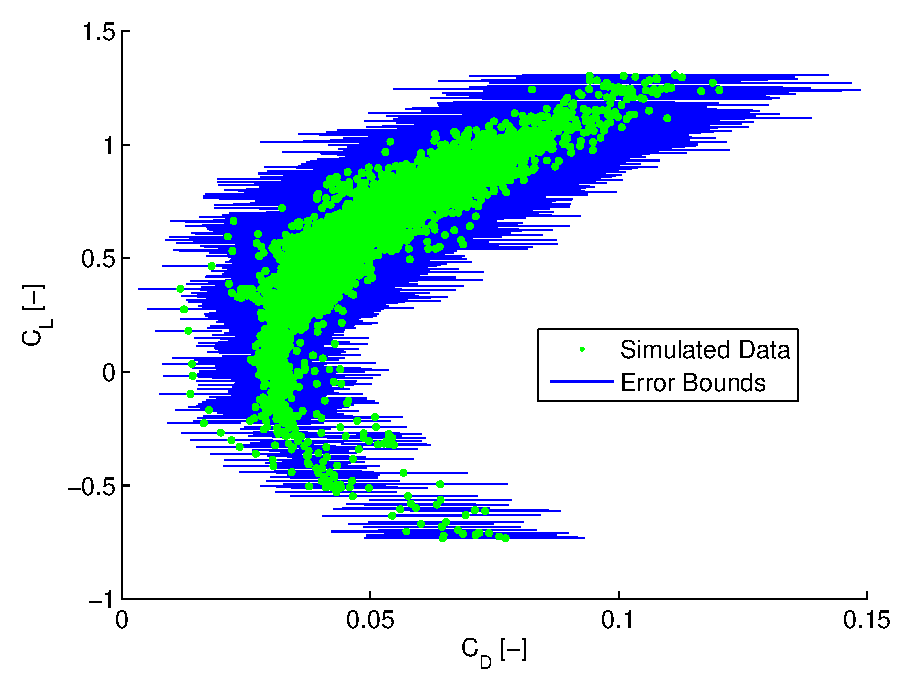
\includegraphics[width=0.5\textwidth]{figures/heteroskedasticity.eps}
      \caption{Heteroskedastic Error from Simulated Flight}
\end{figure}


%todo:cite the fact that heteroskedasticity does not color the estimate
While heteroskedasticity does not color the estimate of $\hat{\beta}_i$, it does color the confidence intervals. The method of dealing with this problem is discussed in Section \ref{leastSquaresError}.


\subsection*{Least Squares Model Error}
\label{leastSquaresError}
The error of a single data point is not the main driving factor in the accuracy of a regression model. The important factors in the model are how accurate the coefficients are known, which is a function of the accuracy of each point, as well as the number of points sampled. The main parameter that describes the accuracy of the regression coefficients are the confidence intervals. A confidence interval is a range of values such that, if the experiment were repeated, the parameter calculated would be within the range some percentage of the time. A parameter can be represented as an estimated value, with a confidence bound

\begin{align}
\label{confidenceInterval}
\beta &= \beta_{EST} \pm t\frac{\sigma}{\sqrt{n}}
\end{align}

where $\beta$ is the parameter in question, $\beta_{EST}$ is the estimated value of the parameter, $t$ is the $t$ value based on the number of samples and the desired confidence interval, $\sigma$ is the standard deviation of the sample, and $n$ is the number of data points collected. Since the number of data points collected during flight will be large ($n>100$), the $t$ value will be taken as 1.96 for a 95\% confidence interval.\\
As previously mentioned in Section \ref{pointErrorSection}, one of the assumptions made in a Least Squares regression is homoskedasticity. However, the error using standard uncertainty propagation is heteroskedastic. This becomes a problem in estimating confidence intervals, because the standard error can be driven by outliers. If each data point had the same error, these outliers could be valid. However, if the data is heteroskedastic, the outlier may have a larger error bound, meaning the data point is not as likely as it first appears. This fact can drive the standard error estimate to be larger than is appropriate, which leads to a larger confidence interval and possibly a false lack of rejection of the confidence interval's hypothesis test. To account for this, the \texttt{robustfit} function in MATLAB  was used to estimate both the coefficients and robust standard error estimates. The \texttt{robustfit} function calculates heteroskedastically-robust standard error estimates by doing a weighted average, where the weighting is based on a radial basis function. This means that the farther away a data point is from the estimated regression model, the less impact it has on the standard error of the model. The default weighting function used by \texttt{robustfit} is bisquare, and it was used for this research.

\subsection*{Kalman Filter Error}
Kalman filters are often used to propagate states. The filter does this by combining the system dynamics with a measured state. The variance is propagated using Equation \ref{kalmanVariance}. When estimating coefficients using the Kalman filter, the $\bar{A}$ state transition matrix is an identity matrix, which is due to the fact that the coefficients stay constant. When propagated through the filter, this means the state estimate $x_k$ is essentially a variance-weighted-average of the coefficient estimates. The matrix $P_k$ contains the variance of the coefficient estimates. Equation \ref{confidenceInterval} calculates the confidence interval of regression coefficients and needs the standard deviation of the mean, also called the standard error. The matrix $P_k$ can be used  to calculate the confidence intervals by noting
\nomenclature{$\sigma$}{Standard deviation}
\begin{align}
P_k &= \begin{bmatrix}
\sigma_{1}^2 &  0  & \ldots & 0\\
0  &  \sigma_{2}^2 & \ldots & 0\\
\vdots & \vdots & \ddots & \vdots\\
0  &   0       &\ldots & \sigma_i^2
\end{bmatrix}
\end{align}

The confidence interval for coefficient $\beta_i$ can be calculated using $\sigma_i$ in Equation \ref{confidenceInterval}.

\chapter{Simulation}
\label{simulation}
\nomenclature{DOF}{Degree of freedom}
A 6-DOF flight simulator was used to validate the drag prediction method before hardware was purchased. The main utility of the simulator was to provide simulated flight test data with signals that contained no errors. The actual sensors used for flight testing contain noise, and this noise can be added onto the pure simulator signals to test the sensitivity of the drag polar regression to sensor accuracy.

\section{Simulation Environment}
The flight simulator used was a model of the de Haviland Beaver that comes as a demo in the Aerospace Toolbox of Simulink. The Simulink model was modified to output required signals to the workspace, which essentially created a sensor with zero noise. The mass, moments of inertia, and reference lengths were then scaled to those of a Zagi R/C aircraft\cite{stevens2003aircraft}. The original Simulink model was already connected to a FlightGear Flight Sim, used as a visualization engine. This model was slightly altered to make flight gauges function properly.

\section{Simulation Inputs}
The engine forces and moments were set to zero in the simulator, to match the assumption of a folding propeller. The drag force calculation built into the Beaver Simulink model was replaced with a parabolic drag polar of the form

\begin{align}
C_D &= C_{D_0} + K_1(C_L(\alpha)-C_{L_{min}})^2+\frac{(C_L(\alpha))^2}{\pi eAR}
\end{align}
\nomenclature{$AR$}{Aspect ratio}
\nomenclature{$C_L$}{Lift coefficient}
\nomenclature{$C_D$}{Drag coefficient}
\nomenclature{e}{Wing lift distribution}
\nomenclature{$C_{D_0}$}{Parasite drag coefficient}
\nomenclature[G]{$\alpha$}{Angle of attack}
Airfoil data, including $K_1$, $C_{L_{min}}$, and $C_L(\alpha)$, was taken from nonlinear aerodynamic data of a NACA 0012\cite{osborne2007transitions}. While this approximation to a real drag polar does not capture the nonlinear section of profile drag rise due to stall, it does represent the limited lifting capability of a real wing.

\section{Simulation Results}
The first goal of the simulation testing was to verify the drag polar equations were correct, and that the data analysis routines developed in MATLAB did in fact match inputs to outputs. The simulation was initialized with various initial states to ensure there was no dependency on initial conditions. The vehicle was then flown by an R/C aircraft pilot using a joystick attached to the simulation. It was noted early in the simulation testing that flying a sweep of speeds was beneficial, as a wider range of the drag polar was flown. This result was included in much of the flight test planning. 

After adequate data had been taken, the data was analyzed without adding simulated sensor noise. The results in Figure \ref{dragPolarNoNoise} show that the equations of motion used in the data analysis functions properly calculate the coefficients being passed into the system.

\begin{figure}[H]
  \centering
    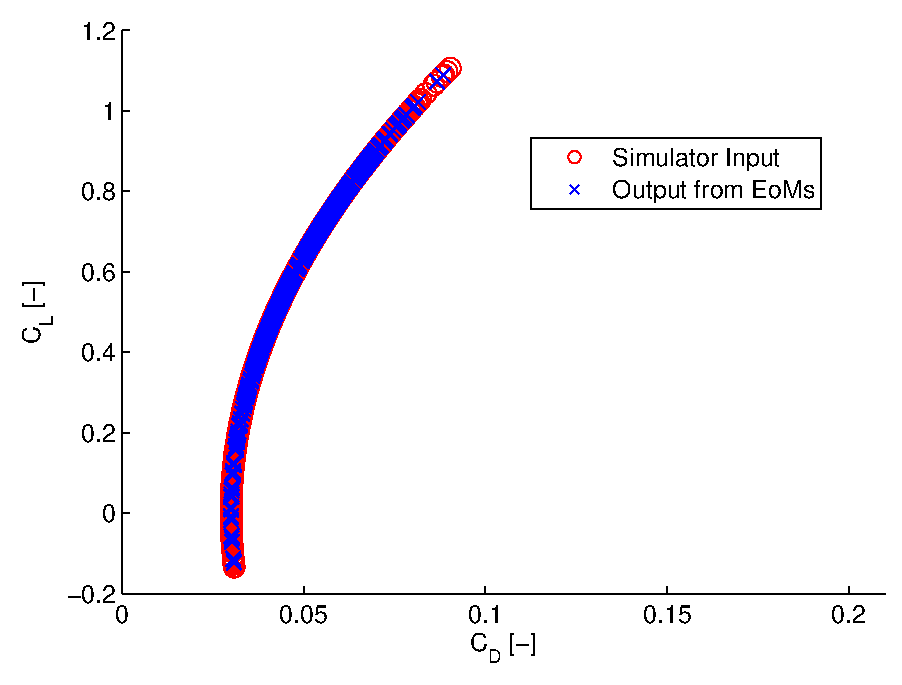
\includegraphics[width=0.5\textwidth]{figures/dragPolarNoNoise.eps}
    \caption{Data Analysis Verification (No Noise)}
        \label{dragPolarNoNoise}
\end{figure}

With this result, noise was added to the system to see how sensitive coefficient estimation was to noise in each sensor. This process was a balancing act between available sensor accuracy and the desired accuracy of the final solution. The final result guided sensor selection to those discussed in Section \ref{hardware}. To check if the final sensors chosen were acceptable, Gaussian noise was added to each state, with a mean of zero and a standard deviation equal to the RMS error listed in the manufacturer's data sheet for each sensor.
\begin{figure}[H]
  \centering
    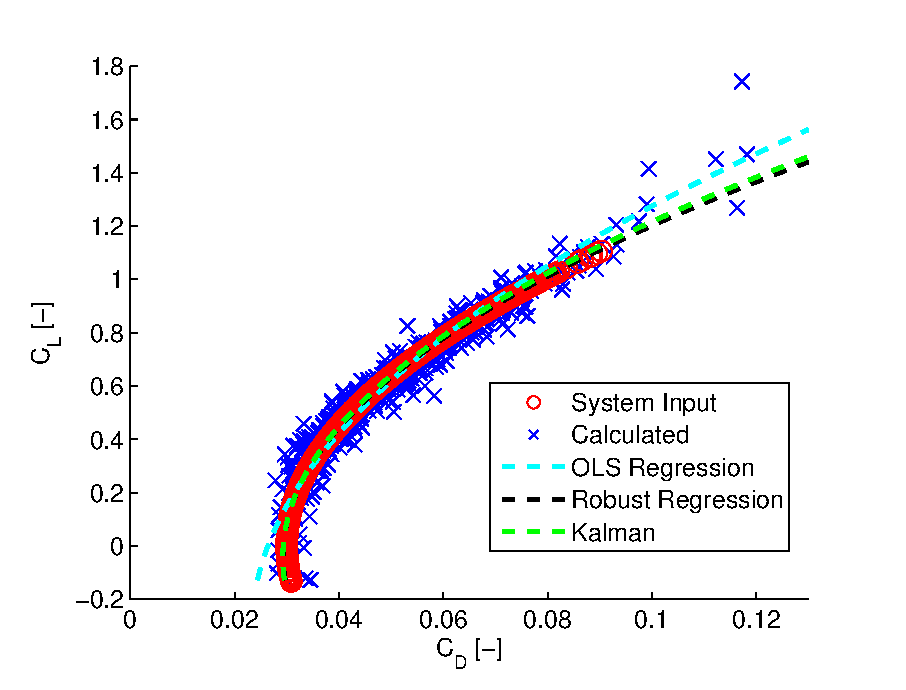
\includegraphics[width=0.5\textwidth]{figures/simDragPolarNoise.eps}
      \caption{Drag Polar Prediction of Simulated Test Flight} \label{dragPolarNoise}
\end{figure}

For the particular simulated test flight shown in Figure \ref{dragPolarNoise}, the estimated drag polar coefficients are shown in Table \ref{simCoeffErrorTable}.

\begin{table}[ht]
\caption{Nonlinear Model Results}
\label{simCoeffErrorTable}
\centering
\begin{tabular}{c c c c}
\hline\hline
 & $C_{D_0}$ & $C_1$ & $C_2$ \\
 \hline
System Inputs & 0.0493 & 0 & 0.03 \\
OLS Estimate & 0.0300 & 0.0196 & 0.0264 \\
Robust LS Estimate & 0.0461 & 0.0034 & 0.0294 \\
Kalman Estimate & 0.0446 & 0.0039 & 0.0293 \\
\hline
\end{tabular}
\end{table}
\nomenclature{OLS}{Ordinary least squares}
\nomenclature{$K_2$}{Drag polar coefficient for $C^2_L$ terms}

The results of this simulated flight test showed that the measurement system outlined in Section \ref{hardware} predicted the simulated drag polar with a reasonable error. It also demonstrates
 the necessity of the heteroskedasticity correction, as the OLS regression has a 65\% error on $K_2$ and a 13\% error on $C_{D_0}$, while the robust regression has a 7\% error on $K_2$ and a 2\% error on $C_{D_0}$.

Since adding random noise results in stochastic error estimates, a Monte Carlo simulation was conducted to quantify expected accuracy values using the sensors selected in Section \ref{hardware}. Error with a standard deviation equal to those reported by the manufacturer was added to clean simulated flight data, and the percent error in each coefficient was saved. This process was repeated 10,000 times, and the results are shown in Figures \ref{fig:cd0monteCarlo}-\ref{fig:c2monteCarlo}.
\begin{figure}[H]
  \centering
    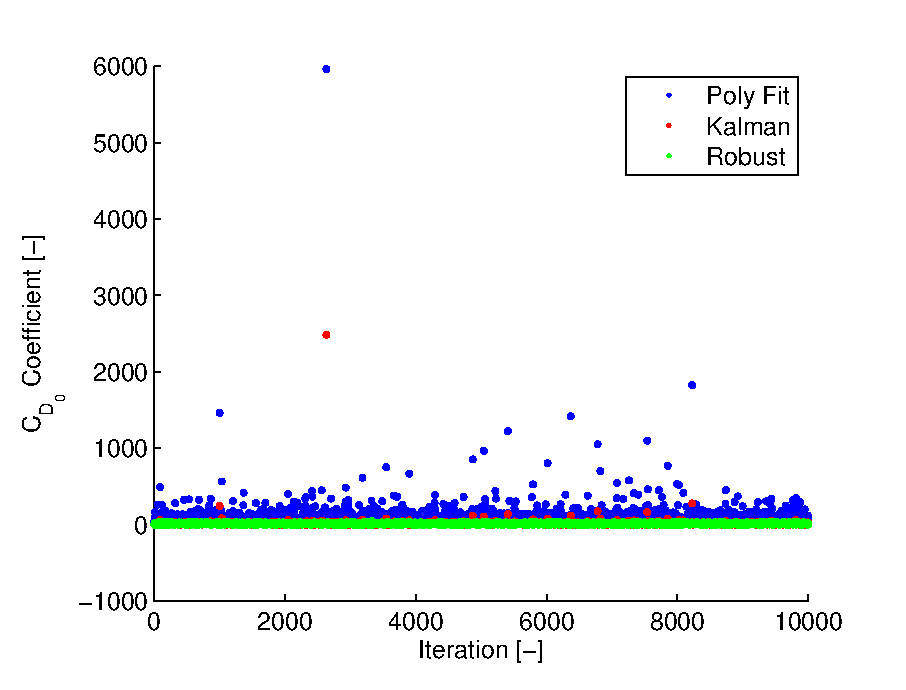
\includegraphics[width=0.5\textwidth]{figures/cd0monteCarlo.eps}
      \caption{$C_{D_0}$ Monte Carlo Simulation}
      \label{fig:cd0monteCarlo}
\end{figure}

\begin{figure}[H]
  \centering
    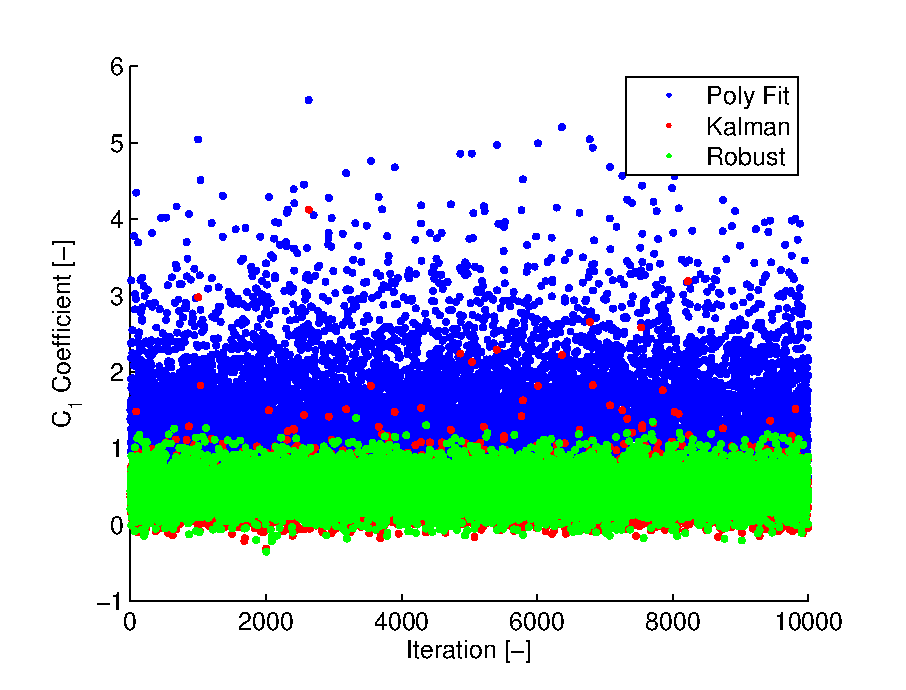
\includegraphics[width=0.5\textwidth]{figures/c1monteCarlo.eps}
      \caption{$C_1$ Monte Carlo Simulation}
      \label{fig:c1monteCarlo}
\end{figure}

\begin{figure}[H]
  \centering
    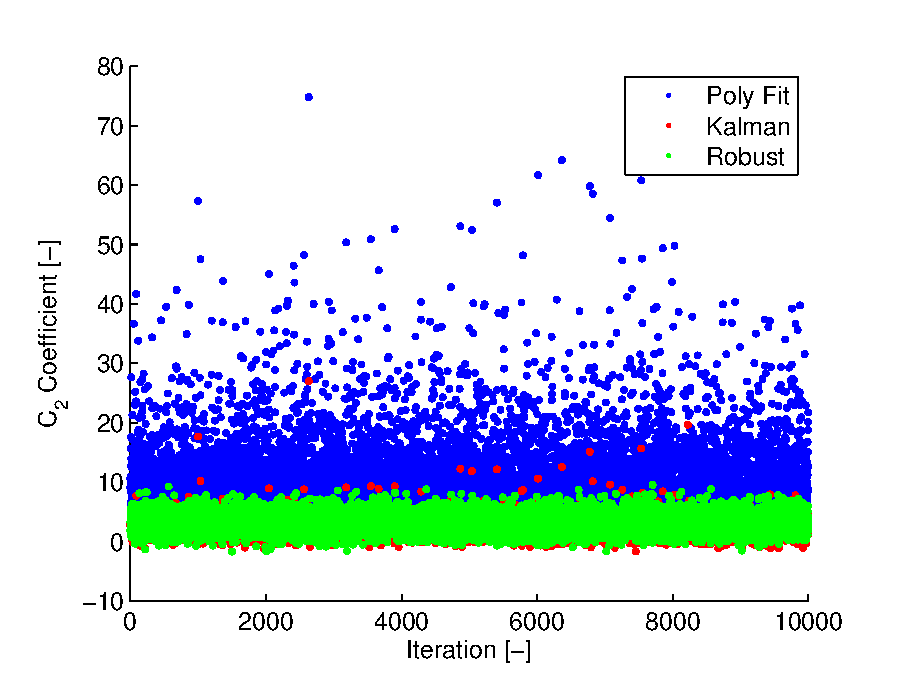
\includegraphics[width=0.5\textwidth]{figures/c2monteCarlo.eps}
      \caption{$C_2$ Monte Carlo Simulation}
      \label{fig:c2monteCarlo}
\end{figure}

The results of the study, summarized in Table \ref{table:monteCarlo}, show that the \texttt{robustfit} regression produced the most accurate and reliable results.

\begin{table}[ht]
\caption{Monte Carlo Results}
\label{table:monteCarlo}
\centering
\begin{tabular}{*7c}
\hline\hline
 &  \multicolumn{3}{c}{Mean Percent Error} & \multicolumn{3}{c}{Percent Standard Error}\\
 & $C_{D_0}$ & $C_1$ & $C_2$ & $C_{D_0}$ & $C_1$ & $C_2$\\
 \hline
OLS & 53.8 & 1.5 & 10.6 & 81.7 & 0.6 & 6.0\\
Robust LS & 12.2 & 0.5 & 3.2 & 6.3 & 0.2 & 1.5\\
Kalman Filter & 12.1 & 0.4 & 2.5 & 26.0 & 0.2 & 1.3\\
\hline
\end{tabular}
\end{table}
\chapter{Hardware}
\label{hardware}
Hardware selection was approached from a ``minimum sensor" perspective. One of the main goals of this thesis was to reduce the number of sensors as much as possible to increase the variety of aircraft the hardware can fly on. To accomplish this, sensors were chosen based on which state they could estimate, with a main goal being to reduce overall size. The sensors were then combined into a single printed-circuit-board (PCB) that eliminated loose wiring and the potential for error that comes with it. 

\section{Flight Computer}
The flight computer chosen was an Arduino Due. This board has a 32-bit ARM processor, 54 digital I/O pins, 12 analog input pins, and 2 analog output pins. The main driver in the decision to use an Arduino-based platform was the vast support community, which allowed quicker code development. The Arduino also offers a package that integrates well into most of the available airframes, and the stacker head pins allowed for easy integration with other boards. The Due in particular was chosen as it is (at the time of writing) the most advanced Arduino available. The main advantages it has over the comparable Arduino Mega is its increased clock speed (84 MHz for the Due\cite{Atmel2012} vs 16 MHz for the Arduino Mega\cite{Atmel2012atmega}) and its 32-bit architecture (vs. 8-bit for the Arduino Mega). The Arduino Due is also capable of some single cycle floating point arithmetic\cite{Atmel2012}, which is another advantage over the Mega.

\begin{figure}[H]
  \caption{Arduino Due Flight Computer} \label{arduinoPicture}
  \centering
    \includegraphics[width=0.5\textwidth]{figures/arduinoDue.jpg}
\end{figure}

The Arduino Due uses a 3.3V architecture instead of the usual Arduino architecture, which uses a 5V operating voltage. This was mainly beneficial, since most of the selected sensors used 3.3V as both supply and logic voltage. An oscilloscope was used to check logic levels of the 5V sensors, and the logical levels were within the Due's voltage limits, so no logic level converters were required. In Due also supplies regulated 5V and passes through the supply power, which must be between 6V and 15V. The board will be powered through the 3.5mm barrel jack, using a 3-cell LiPo battery, with a nominal voltage of 11.1V.

\section{Accelerations}
The accelerometer chosen for this thesis was the ADXL-362 from Analog Devices. It has a noise error of $175\mu\text{g}/\sqrt{\text{Hz}}$ and uses a 3.3V digital SPI interface\cite{adxl362DataSheet}. The accelerometer is in a QFN package and was surface mounted to the main PCB, with a decoupling capacitor between power and ground. The circuit was modeled after Sparkfun's ADXL-362 Breakout Board\cite{Sparkfunadxl362BOB}.
%todo: add picture of Eagle schematic for accelerometer.

\section{Vehicle Mass}
All test vehicles will be weighed using a U-Line H-1650 counting scale. The scale has an accuracy of 0.001 lbs and a maximum capacity of 30 lbs. The minimum capacity of the scale is 10 grams \cite{U-Line}.
\section{Euler Angles}
The Euler angles of the aircraft can be estimated using either an 3-d electronic compass or a 3-d magnetometer. A magnetometer reads the direction and magnitude of a magnetic field, while a compass combines a magnetometer with accelerometer readings to produce a more accurate estimate of the true angles. However, if the vehicle is maneuvering, the craft's acceleration will distort the angle estimation, making compasses unsuitable for this application. A Honeywell HMR-2300 3-d magnetometer was used for this thesis. 

\begin{figure}[H]
  \caption{Honeywell HMR-2300 3-d Magnetometer } \label{hmr23000Picture}
  \centering
    \includegraphics[width=0.5\textwidth]{figures/hmr2300.jpg}
\end{figure}

This magnetometer provides a RMS error of 0.01 Gauss for all axes, using the 1 Gauss full-scale setting\cite{hmr2300DataSheet}. 

The HMR-2300 can be supplied with power between 6V and 15V, so the 3-cell 11.1V nominal LiPo battery that powers the Arduino also passes through to power the magnetometer. Additionally, the HMR-2300 operates using an RS-232 serial interface. To properly interface with the Arduino Due, which uses 3.3V TTL logic levels, a Max-3232 integrated circuit (IC) was used. This IC, when combined with charge pump capacitors, translates TTL levels between 3V and 5.5V to RS-232 logic levels of $\pm6$V.
%todo: include schematic of HMR2300 board
 This board was connected to the magnetometer using a DB-9 connector, and was connected to the flight computer using an RJ-11 cable.
\subsection*{Euler Angle Kalman Filter}
For increased accuracy, a discrete linear Kalman filter is applied. This necessitated adding a three-axis gyroscope to the system. The gyroscope chosen was the Invensense ITG-3200, which comes in a QFN package. This gyroscope has a total error of $0.38^\circ/$s-rms\cite{itg3200DataSheet}, and uses a digital I$^2$C interface on a 3.3V operating voltage. The gyroscope has a full-scale span of $\pm2000^\circ/$s. The gyroscope was integrated into the main sensor board using a circuit based on that of Sparkfun's ITG-3200 breakout board\cite{itg3200BOBSchematic}.

%todo: add eagle schematic of gyro circuit

With the angular rates available from the gyroscope, the system equations for the Kalman filter are
\begin{align}
\begin{bmatrix}
\phi_{k}\\
\theta_{k}\\
\psi_{k}
\end{bmatrix} & = \begin{bmatrix}
1 & 0 & 0\\0 & 1 & 0\\0 & 0 & 1
\end{bmatrix}\begin{bmatrix}
\phi_{k-1}\\
\theta_{k-1}\\
\psi_{k-1}
\end{bmatrix}
+ \begin{bmatrix}
\Delta T & 0 & 0 \\ 0 & \Delta T & 0\\0 & 0 & \Delta T
\end{bmatrix}\begin{bmatrix} 
p_k \\ q_k \\ r_k 
\end{bmatrix}+\hat{w}_{k-1}\\
z_k & = \begin{bmatrix}
1 & 0 &0\\0&1&0\\0&0&1
\end{bmatrix}\begin{bmatrix}
\phi_{k}\\
\theta_{k}\\
\psi_{k}
\end{bmatrix}+\hat{v}_{k-1}
\end{align}

The measurement covariance noise matrix was calculated using the standard deviation of the calibration data for the magnetometer, and the process noise covariance matrix was calculated using the standard deviation of the calibration data for the rate gyroscope.

\section{Wind Angles}
The accuracy at which the aerodynamic wind angles are calculated is critical to the overall prediction accuracy. In keeping with the goal of minimizing the number of required sensors, an attempt was made to estimate aerodynamic angles without directly measuring them. There has been a plethora of work conducted on this subject. One of the first available papers on the subject was from the Air Force Institute of Technology \cite{joseph1988}. In that paper, two methods were developed: one for in flight estimation, and the other for post-flight estimation. Both methods relied on either estimated or known stability derivatives. Since the purpose of this thesis is to estimate part of the dynamics, this estimating scheme will not work. Other techniques assume linearization about an operating condition \cite{morelli2012real}. For R/C aircraft this assumption generally cannot be made due to visual flight rules. Other work \cite{Lie2013} combined a dynamics model and a no-vertical-wind assumption. The overarching theme of this previous estimation work was that too many assumptions needed to be made to get results that were not accurate enough ($\approx1^\circ-2^\circ$) for drag polar estimation. For this reason, it was necessary to directly measure airflow angles.

\indent
A five-hole probe was chosen to measure aerodynamic angles as they do not contain moving parts and can provide very accurate, repeatable data. The five-hole probe selected was the Aeroprobe Air Data probe. It has a length of 6 inches and a diameter of 1/8 inch and comes calibrated to pressures. Each pair of lines of the air data probe is connected to an All Sensors digital differential pressure sensor with a full scale range of $\pm$5"-H$_2$O\cite{allsensorsDDO}.

\begin{figure}[H]
  \caption{All Sensors 5-INCH-D-DO Pressure Sensor} \label{allsensorsPressurePic}
  \centering
    \includegraphics[width=0.5\textwidth]{figures/allsensorsPressure.jpg}
\end{figure}

These pressure sensors have a total error band of 0.25\% of full scale. They use a UART serial interface that operates on a 5V logic level, but the logic levels are compatible with the 3.3V interface of the Arduino Due. The serial interface includes addressable read commands, which allows multiples devices on a single bus, and ensures all devices record pressure at the same time. The sensor can output both a 14-bit pressure reading and a 12-bit temperature reading, which the devices uses to correct its pressure measurement.

\subsection{Calibration}
The five-hole air-data probe is calibrated using a Cal-Jet.

\subsection{Wind Angle Kalman Filter}

To improve the accuracy of the wind angle estimation, a discrete Extended Kalman filter was used. The state transition functions are nonlinear and are
\begin{align}
\dot{\alpha} & = \frac{1}{V\cos\beta}(-a_x\sin\alpha+a_z\cos\alpha)+q-(p\cos\alpha+r\sin\alpha)\tan\beta\\
\dot{\beta} &=\frac{1}{V}(-a_x\cos\alpha\sin\beta+a_y\cos\beta-a_z\sin\alpha\sin\beta)+p\sin\alpha-r\cos\alpha
\end{align}

These state transition equations come from solving for the vehicle forces in wind axes instead of body axes\cite{klein2006aircraft}. The equations for the Kalman filter for the wind angles are
\begin{align}
\begin{bmatrix}
\alpha_k\\\beta_k
\end{bmatrix} &= \begin{bmatrix}
1& 0\\0&1
\end{bmatrix}\begin{bmatrix}
\alpha_{k-1}\\\beta_{k-1}
\end{bmatrix}+\begin{bmatrix}
\Delta T& 0\\0&\Delta T
\end{bmatrix}\begin{bmatrix}
\dot{\alpha_{k}}\\\dot{\beta_{k}}
\end{bmatrix}+\hat{w}_{k-1}\\
z_k & = \begin{bmatrix}
1 & 0\\0&1
\end{bmatrix}\begin{bmatrix}
\alpha_{k}\\
\beta_{k}
\end{bmatrix}+\hat{v}_{k-1}
\end{align}

The process covariance matrix was calculated using the error propogation discussed in Section \ref{pointErrorSection} and the standard deviation data from calibration of each of the sensors. The measurement noise covariance matrix was calculated based on the standard deviation data for the 5-hole probe calibration.


\section{Additional Sensors}
A uBlox LEA-6T GPS receiver was included in the data acquisition system to aid in mission visualization. This model was selected for its ability to output raw timing data, which can potentially be used to get an extremely accurate inertial velocity estimate\cite{ubloxDemo}. The receiver itself was integrated onto a board sold by CGS Shop and has UART,USB, and I$^2$C interface options. 

\begin{figure}[H]
  \caption{CGS Shop Board for uBlox LEA-6T} \label{gpsPicture}
  \centering
    \includegraphics[width=0.5\textwidth]{figures/gpsBoard.jpg}
\end{figure}

A barometric altitude sensor was also included the data acquisiton system. The model chosen was an All Sensors BARO-DO, which has a range of 600 mBar to 1100 mBar\cite{allSensorsBaroDatasheet}. It has a nominal error of 1.0 mBar. It has the same packaging and communication protocol as the All Sensors 5-INCH-D-DO used for wind angle measurement, which simplified integration.

A digital temperature sensor was combined with the barometric altitude sensor to estimate the air density.
\begin{figure}[H]
  \caption{Dallas Semiconductors' DS18B20 Digital Temperature Sensors} \label{ds18b20Picture}
  \centering
    \includegraphics[width=0.25\textwidth]{figures/ds18b20Picture.jpg}
\end{figure}
 The DS18B20 from Dallas Semiconductors was chosen for its relatively simple One-Wire interface. The device can be powered with the communication line and has a $\pm$0.5$^\circ$C nominal accuracy\cite{DS18B20Datasheet}.

Header pins capable of reading commanded PWM signals to servos were also added. Future work could include stability derivative estimation, and the header pins provide PWM measurement, which can map to servo angles, if it is assumed the servo is not stalled. 

\subsection{Data Acquisition Integration}
The hardware was initially built using a breadboard to ensure proper connections and to develop software. Once completed, sensors were packaged into a shield for the Arduino. This shield plugs directly into the Arduino, eliminating the need to disconnect and reconnect wiring. A board responsible for interfacing the main sensor board with the HMR-2300 was also developed, and connects to the main board with an RJ-11 cable. This allows the magnetometer to be placed with relative freedom within a vehicles fuselage. A third board was developed to integrate the pressure sensors with the main sensor board. This pressure board can be located near a wing tip and  provides expandability should additional sensors be desired in the future. It also interfaces the temperature sensor. Finally, all data was saved to a microSD card attached to the main sensor board. Data was saved in binary format for both increased speed and file size reductions. Once on the ground, the data is converted to meaningful values using a MATLAB parser.

%\chapter{Flight Test}
\label{sect:flightTestSec}
Flight testing was done at Cal Poly's Educational Flight Range (EFR). The goal of flight testing was to validate the performance of the final system design. The drag polar estimation was chosen as the validation case, and was approached from each of the three coefficients. To this end, the final system was flown on multiple vehicles which each had a different role in the validation routine.

\section{$C_{D_0}$ Validation}
Validation of the parasite drag coefficient was completed using a Finwing Universal Penguin FPV R/C aircraft\cite{penguinRC}. 

%todo: add picture of penguin plane
This model was selected because it has a large internal payload bay which has plenty of room for the system and had enough excess power to overcome additional drag. The validation method involved flying the base model and measuring the drag polar. Then, parasite drag was added in the form of streamers, similar to those used in amateur rocketry recovery. The benefit of this technique is that it does not modify either of the other two drag polar coefficients. A power law fit to the expected drag coefficient of the streamers was given in \cite{Auman2001}. The validation routine was flying the vehicle with and without streamers and seeing the horizontal shift in the drag polar.

\section{$K_1$ Validation}
The $K_1$ term of the drag polar is mainly driven by the $C_L$ for minimum drag. To validate this coefficient, a custom test vehicle was manufactured with two different wings of equal area. One wing had a NACA 63-014 airfoil cross section, which is a symmetric airfoil, meaning the vehicles $K_1$ value should be zero. The next wing had a NACA 63-614 airfoil, which has a design $C_L$ for minimum drag of 0.6. The validation method was flying both of these wings on the same vehicle, and seeing the vertical shift in the drag polar.
\section{$K_2$ Validation}
The $K_2$ drag polar coefficient is the inviscid drag due to lift term. This form of drag comes from the wing tip vortices of a finite wing, and is affected by both wing aspect ratio and lift distribution. Prandtl showed experimentally\cite{prandtl1923applications} that, for rectangular wings with aspect ratios between one and seven, the drag coefficient corresponding to one aspect ratio can be scaled to that of a different aspect ratio using the equation

\begin{align}
C_{D,1} &= C_{D,2} + \frac{C^2_L}{\pi e}(\frac{1}{AR_1} - \frac{1}{AR_2})
\end{align}

The $K_2$ validation uses this fact by flying the same test aircraft with two different sets of wings with the same area. The first wing has an aspect ratio of three, while the second wing has an aspect ratio of seven. The $AR = 3$ wing was then corrected to the $AR = 7$ wing and the resulting drag polar should fall on top of each other.
\chapter{Results}
\label{results}
The system was built and tested to prove functionality. After functionality testing was complete, the system was integrated into a 0.40-size Piper Cub R/C aircraft.

\begin{figure}[H]
\label{sysIntPics}
\begin{center}
\begin{minipage}[b]{0.45\linewidth}
  \centering
    \includegraphics[width=0.9\textwidth]{figures/sysInt1.jpg}
\end{minipage}
\begin{minipage}[b]{0.45\linewidth}
  \centering
    \includegraphics[width=0.9\textwidth]{figures/sysInt2.jpg}
\end{minipage}
\end{center}
\caption{System Integration into 0.40-size R/C Piper Cub}
\end{figure}
After integration, an initial test flight was conducted. Unfortunately, an electrical short-circuit caused the vehicle to  crash and corrupted some data, so no aerodynamic force estimation has been conducted. However, the micro-SD card did survive the crash, and provided enough data to show the system was collecting data as expected before the short-circuit.
\begin{figure}[H]
\label{sysIntPics}
\begin{center}
\begin{minipage}[b]{0.4\linewidth}
\label{preFlightFig}
  \centering
    \includegraphics[width=0.9\textwidth]{figures/preFlight.jpg}
    \caption{Pre-Flight System Checks}
\end{minipage}
\begin{minipage}[b]{0.4\linewidth}
  \centering
    \includegraphics[width=0.9\textwidth]{figures/crash.jpg}
    \caption{Crashed Vehicle in Water}
\end{minipage}
\end{center}
\end{figure}

 The small amount of data collected was analyzed using a user interface developed to rapidly process the data acquisition system's files. This user interface will allow designers to analyze data immediately following a test flight and make corrections to the test flight program while still at the test flight location.
\chapter{Summary}
\label{summary}
A flight data computer capable of measuring a small UAVs aerodynamic forces was developed. The system utilizes an Arduino Due as the main flight computer, and integrates both sensors necessary for aerodynamic force calculation, and additional sensors that provide interesting information about the vehicle. The system was manufactured in a PCB form to keep reliability high, integrated into a 0.60-size electric Piper Cub, and validated for accuracy and repeatability. The flight tests showed a $C_{D_0}$ accuracy of 6\% of the trailing cone's estimated drag coefficient, and a zero lift angle of attack accuracy of less than 1\% error compared to that estimated by XFOIL. The lift curve slope estimated from combining flight data with XFOIL analysis was, on average, accurate to 17\%, which indicates proper lift distribution estimation. Future work could include a sensor fusion algorithm, which would be developed to combine inertial sensors with the air data system and other available sensors in a manner similar to other current research,\cite{wvINSAirData}$^,$\cite{gtUKF} thus giving full situational awareness to the UAS. This situational awareness could allow stability and control derivative estimation, which the aircraft designer could use to size tail and control surfaces. In-flight dynamic thrust estimation is also possible, and could be validate against propeller data available from the University of Illinois at Urbana-Champagne.\cite{brandt2011propeller} Of most interest to the other, future work could utilize this thesis to estimate the lift and drag impact of difference vehicle configurations to quantitatively make trade studies early in the conceptual design phase. This could include configuration level trades, or subsystem level (no landing gear, normal gear, gear with wheel pants, retractable gear,etc.) trade studies, which could dramatically increase the current small scale aerodynamic knowledge base at Cal Poly.
%\section{Future Work}
The accuracy of the system developed still needs to be extensively validated. The immediate future work following this paper will be quantifying the accuracy of the system, as well as verifying reliability and safe integration into multiple UASs. Most of the accuracy estimation will be accomplished by measuring changes to a vehicle's drag polar. Parasite drag will be proven by adding a known quantity and measuring the change in the parasite drag coefficient of the test vehicle. To quantify the accuracy of drag-due-to-lift, wings with different aspect ratios will be used on the vehicle, which should combine into a single equivalent curve\cite{prandtl1923applications}. Following the accuracy estimation, a sensor fusion algorithm will be developed to combine inertial sensors with the air data system and other available sensors in a manner similar to other current research,\cite{wvINSAirData}$^,$\cite{gtUKF} in order to give full situational awareness to the UAS. This situational awareness could allow stability and control derivative estimation, which the aircraft designer could use to develop and simulate new control laws using actual stability derivatives.
% ------------- End main chapters ----------------------
\clearpage
\begin{appendices}
\chapter{Data Acquisition System Usage}
This section documents the steps required for correct usage of the data acquisition system.

\section{Integration}
The main data acquisition system should be integrated into the flight test vehicle near the vehicle's center of gravity.\nomenclature[A]{CG}{Center of gravity} The system should have one of its principal axes lined up roughly parallel to the vehicle's longitudinal axis. Servos should be connected to both the main board and the aircraft's receiver using a y-splitter with 2 male and one female connectors. If applicable, the servos should be connected according to the Table \ref{table:servoSetup}.
\begin{table}[ht]
\caption{Air Data System Setup}
\centering
\begin{tabular}{c c}
\hline\hline
 Servo & PWM Pinout\\
\hline
Throttle & D37\\
Elevator & D38\\
Rudder & D39\\ 
Aileron (1/2) & D40\\
Aileron (2/2) & D41\\
Gear & D42\\
Auxiliary (1/2)& D43\\
Auxiliary (2/2)& D44\\
\hline
\end{tabular}
\label{table:servoSetup}
\end{table}

If the additional digital pin-outs are being use for measuring servo signals, the ``+V'' jumper should not have a jumper on it. If using the digital pin-outs to run digital sensors or command servos, place the jumper on the appropriate voltage level setting.

The data acquisition system is powered through the barrel jack on the Arduino Due. The recommended operating voltage is between 7V and 12V, with an absolute maximum of 16V. The power can be supplied using either a battery dedicated to the data acquisition system, or through a BEC from the ESC. If using the ESC's BEC, set the BEC output somewhere between 7V and 12V. \textbf{CRITICAL:} ensure the red wire from the ESC does not pass to the receiver, as it is over-voltage for standard R/C equipment.\nomenclature[A]{ESC}{Electronic speed controller}\nomenclature[A]{BEC}{Battery elimination circuit}

The pressure board can be placed anywhere in the vehicle, as long as it can be connected to the main board. The pressure sensors should be attached to the five-hole probe as follows:

\begin{table}[ht]
\caption{Air Data System Setup}
\centering
\begin{tabular}{c c c c}
\hline\hline
 Pressure Sensor & Port A & Port B & Measurement\\
\hline
0 & Tube 5 & Tube 4 & $\beta$ \\
1 & Tube 6 & Tube 1 & $q_{\infty}$\\
2 & Tube 3 & Tube 2 & $\alpha$\\ 
3 & n/a & Tube 6 & $P_S$\\
\hline
\end{tabular}
\label{table:airDataSetup}
\end{table}
\nomenclature[A]{$P_S$}{Static pressure}

Port A and Port B refer to the ports as labeled in Figure \ref{fig:pressureLabels}, and the tube number refers to the five-hole probe tubes. These tube numbers increase as the tube length decreases: Tube 1 refers to the longest tube, Tube 6 refers to the shortest tube.

\begin{figure}[H]
  \centering
    \includegraphics[width=0.5\textwidth]{figures/allsensorsPressureLabeled.jpg}
      \caption{Port Description for Pressure Sensors} \label{fig:pressureLabels}
\end{figure}

The pressure tubing and temperature sensor line should be routed together to the air data boom and secured for flight. The temperature sensor's wiring is a standard servo extension. The air data boom's accelerometer wiring is a standard RJ-25 \textit{patch} cable and should be routed in a separate bundle, as it will be removed before flight.

The air data boom itself should be integrated as far from aerodynamic effects as possible. For this thesis, the boom was mounted roughly one chord length in front of the leading edge of the wing and approximately halfway down the wing span. Other mounting locations could include out the aircraft's nose for a pusher vehicle, or on the vertical tail. The aluminum block accepts a 0.25" carbon fiber tube as it's mounting interface, and this tube should be mounted roughly in-line with the airflow angle expected during flight. The temperature sensor can be taped to the tube.

\section{Pre-flight Procedure}
\label{sect:preFlightProc}
The pre-flight procedure in this section must be completed in addition to all preparation listed in Section \ref{sect:flightTestDocs}.

\begin{enumerate}
\item With the transmitter turned on, power on the receiver.
\item Plug in the micro-USB cable into the main data acquisition board.
\item Ensure the micro-SD card is empty and formatted as FAT32, then insert it into the main data acquisition board.
\item Plug in the main data acquisition system's battery pack or the BEC. \textbf{CRITICAL:} ensure the red wire does not connect the BEC to the receiver.
\item Plug the pressure sensor board into the main data acquisition board.
\item Plug in the air data system's RJ-25.
\item Upload the calibration routine to the main board, and follow the prompts to calibrate the gyroscope, accelerometer, and magnetometers.
\item Place a wind blocker (Daisy/Solo cups work) over the five-hole probe and calibrate the pressure sensors, using the calibration routine.
\item Load the main data acquisition script onto the main data acquisition board.
\item Turn on serial output and check that all sensors are functioning properly.
\item Initialize the micro-SD card.
\item Turn off serial output.
\item Turn on data logging and verify the system is saving data.
\item Remove the micro-USB cable and the air data system's RJ-25 cable.
\item Plug in the main propulsion battery pack.
\end{enumerate}
The data acquisition system is now ready for flight.

\section{Flight test plan}
When using the data acquisition system for drag polar estimation, a better model estimate is possible with proper flight maneuvers. The main technique to improve the model is to vary speeds as much as possible, which allows more of the drag polar to be flown. Multiple glides that begin at the highest speed possible should be completed. To achieve the highest initial gliding speed, the aircraft should be put into a dive at full throttle, with plenty of available altitude. Throttle should then be cut, and the dive should briefly continue. After a few seconds of diving, the aircraft should be leveled off and altitude should be maintained, until the vehicle stalls. Repeating this process will provide a large sweep of the flight envelope.

Inverted flight can also help fill out the section of the drag polar that occurs below $C_{L_{min}}$. However, inverted flight should occur at high speeds, to avoid the nonlinear section of the inverted airfoil.

\section{Post-Flight}
Immediately after the vehicle lands, the vehicle's propulsion pack should be unplugged. Next, unplug the data acquisition system's battery pack, remove the micro-SD card, and save the data to a computer. Optionally, after the flight is complete, a second round of zero offset calibration data may be acquired. This set ensures that any drift that occurred during the flight is accounted for.

Once the data is saved to a computer, the data analysis GUI can be used to quickly process the data. \nomenclature[A]{GUI}{Graphical user interface} The user interface can estimate a drag polar using the following steps:
\begin{enumerate}
\item Run \texttt{fileReader.m}.
\item Click the ``Load Data'' button to load flight data. If you'd like an ASCII data file, choose yes on the prompt.
\item Select the pressure calibration file.
\item Select the accelerometer/gyroscope calibration file.
\item Select the magnetometer calibration file.
\item Select the air data system alignment calibration file.
\item Input the reference area in the $S_{REF}$ box and the weight in the Weight box.
\item Click ``Ignore Data With Thrust.''
\item Click ``Display'' in the Quadratic Fit box.
\end{enumerate}

Google Earth plots are also available by clicking the ``Google Earth'' button. The ``X Axis'' and ``Y Axis'' drop down menus are also available, which allows any signal to be plotted against any other signal.

\section{Embedded Software Protocol}
The main data acquisition code allows the user to interface with the Arduino through a serial text interface. A list of available commands for the main data acquisition script, along with their intended functions, is shown in Table \ref{table:mainScriptComms}.
\begin{table}[H]
\caption{Available Commands for \texttt{mainScript.ino}}
\centering
\begin{tabular}{|c | c|}
\hline
 Command & Utility\\
 \hline\hline
dataOn & Turn on data logging to SD card\\\hline
dataOff & Turn off data logging to SD card\\\hline
initSD & Initialize SD card\\\hline
serialOn & Turn on serial output\\\hline
serialOff & Turn off serial output\\\hline
? & Help menu\\\hline
\end{tabular}
\label{table:mainScriptComms}
\end{table}

Note that all commands must be sent with a start character (`\texttt{\#}') and an end character (`\texttt{\&}'.) A proper command to turn on serial output would then be \texttt{`\#serialOn\&'}.

The calibration code also interfaces with the Arduino using a text interface. The calibration script's commands are shown in Table \ref{table:calibComms}.
\begin{table}[H]
\caption{Available Commands for \texttt{calibration.ino}}
\centering
\begin{tabular}{|c | c|}
\hline
 Command & Utility\\
 \hline\hline
accelGyro & Calibrate accel for slope and offset, gyro for offset, and probe alignment. 
Saved to \texttt{ACCLGYRO.clb}.\\\hline
pressure & Calibrate offset of pressure sensors. 
Saved to \texttt{PRESSURE.clb}.\\\hline
mag & Calibrate magnetometers for hard- and soft-iron effects. 
Saved to \texttt{MGNTMTRS.clb}.\\\hline
? & Help menu\\\hline
\end{tabular}
\label{table:calibComms}
\end{table}

Note that, like the main script, all commands must be sent with a start character (`\texttt{\#}') and an end character (`\texttt{\&}'.) A proper command to calibrate the air data system alignment would then be \texttt{`\#accelAlign\&'}.
\chapter{Wiring Schematics}
The following documents the wiring of the circuit boards. The actual Eagle files are available in \texttt{\textasciitilde/eagle/}.
\begin{figure}[H]
  \caption{Arduino Due Flight Data Recorder v3.20BOB Schematic} \label{fig:thesisSchematic}
  \centering
    \includegraphics[width=0.7\textwidth]{figures/thesisSchematic.eps}
\end{figure}

\begin{figure}[H]
  \caption{Arduino Due Flight Data Recorder v3.20BOB Layout} \label{fig:thesisBrd}
  \centering
    \includegraphics[width=0.6\textwidth]{figures/thesisBrd.eps}
\end{figure}

\begin{figure}[H]
  \caption{Pressure Board v2.20 Schematic} \label{fig:satelliteSchematic}
  \centering
    \includegraphics[width=0.8\textwidth]{figures/satellitev2Sch.eps}
\end{figure}

\begin{figure}[H]
  \caption{Pressure Board v2.20 Layout} \label{fig:satelliteBrd}
  \centering
    \includegraphics[width=0.7\textwidth]{figures/satellitev2Brd.eps}
\end{figure}

\chapter{Flight Test Procedure}
\label{sect:flightTestDocs}
This section documents proper flight test procedure, which has been learned from extensive flight testing experience and many crashed vehicles. It is split into three main time periods:
\begin{enumerate}
\item Pre-Flight Preparation
\item Flying Field Procedure
\item Post-Flight 
\end{enumerate}
The testing procedure is split into these time categories to ensure the testing is efficient and that any unforeseen circumstances can be dealt with quickly. Specifically , this guide applies to the Cal Poly Flight Lab testing a vehicle at the Cal Poly Educational Flight Range.

\section{Pre-Flight Preparation}
The preparation work required for a test flight is often overlooked, and this section will document how to effectively prepare to flight test a vehicle. The main purpose of pre-flight preparation is to minimize the possibility of problems that might force a test to be canceled after already going to the field.
\subsection{Day Before Test}
The days before a flight test are critical to ensuring the test is completed successfully. The following should be done at least one day before the the test is scheduled:
\begin{enumerate}
\item Charge all flight battery packs, including any receiver or auxiliary packs.
\item Charge the transmitter battery.
\item Ensure the airframe is structurally sound (wing tip test minimum.)
\item Verify radio system communicates properly, and the correct fail-safe is in place. \textbf{Important}: If the receiver has been used by Design/Build/Fly, the fail-safe must be changed to normal mode.
\item Verify control surface deflections matches desired directions, and all radio mixes work.
\item Verify the motor/propeller spin in the correct direction.
\item Pack a flight box, containing any necessary tools (recommend: screw drivers; masking, painter's, and strapping tape; razor blades; CA glue and kicker; spare propellers; paper and pencil; as a minimum.)
\item Check the weather. The closest monitoring station to the field is \href{http://www.wunderground.com/cgi-bin/findweather/getForecast?query=35.326\%2C-120.738\&sp=KCASANLU17}{KCASANLU17}.It is generally better to flight test early in the morning, since there will be less people at the field, winds will be calmer, and the sun won't be as harsh in the pilot's eyes.
\item Check the SLO Flyers' flight schedule. Some days are reserved for certain events (glider competitions, etc.) and these need to be worked around.
\item Make sure all required personnel know when and where to meet, and there is sufficient transportation to get to the field.
\item Create flight documentation that clearly lays out the test goals and how they will be accomplished. Print copies for all personnel.
\end{enumerate}
\subsection{Day Of Test}
The morning of the flight test, the person responsible for the test should arrive early enough to accomplish the following, before leaving campus:
\begin{enumerate}
\item Pack flight batteries into flight box, including receiver and auxiliary packs.
\item Pack battery charging equipment, with adapters and leads, if necessary.
\item Pack transmitter into box.
\item Double check control surface deflections and radio link.
\item Do a full system check, potentially including a short taxi test in the quad.
\item Do a final check that all equipment made it into vehicles, before leaving the lab.
\end{enumerate}

\section{Flying Field Procedure}
With the pre-flight preparation completed, the testing at the flying field should be fairly event free. Any problems that occur should be either fixable with the minimum supplies in the flight box, or the test should be canceled to minimize risk, and repairs done at the lab. Specific procedures at the flight field will depend on the test being conducted, but below are steps that apply to nearly all tests before flight.
\begin{enumerate}
\item Verify structural integrity using a wing tip test.
\item Verify motor/propeller are spinning in the correct direction.
\item Verify control surface deflections match desired directions.
\item Verify radio link and fail safe mode by completing a range check.
\item Verify center of gravity is at an appropriate location.
\item Create flight timer on the transmitter so the pilot knows how long the aircraft has been flying.
\item Document any required data before the flight, such as aircraft weight and geometry.
\item Document current weather conditions (wind speed and direction, temperature, humidity, barometric pressure) using the Kestrel portable weather station.
\end{enumerate}

\section{Post-Flight}
Upon successful completion of a flight test, all data should be saved to a computer. The flight test cards, pre-flight data documentation, and any notes should be scanned and saved with the flight data. This data should be archived in a .zip file, with the date attached.

If the test flight resulted in a crash, any available data should still be saved. Any video or pictures of the flight should be saved as well, to aid in isolating what caused the crash. If useful, pictures should be taken of the crash site. Afterwards, all pieces of the aircraft should be returned to the lab, where the root cause of the accident should be determined.

After the root cause has been determined, remove all electronics from the vehicle, including batteries, speed controller, motor, servos, and receiver. If the vehicle was a complete loss or went into water, through these components away: \textbf{do not} return to lab supplies. If the vehicle was not a complete loss, verify all components work properly.
%\chapter{$C_{D_0}$ Flight Test Card}
%\chapter{$K_2$ Flight Test Card}
\chapter{Sample System Ouput}
This appendix contains graphs representing typical outputs from the data acquisition system, shown in strip chart format.
%\section{Sample System Ouput - Raw Data}
\begin{figure}[H]
	\centering
	\caption{accelX vs. Time}
		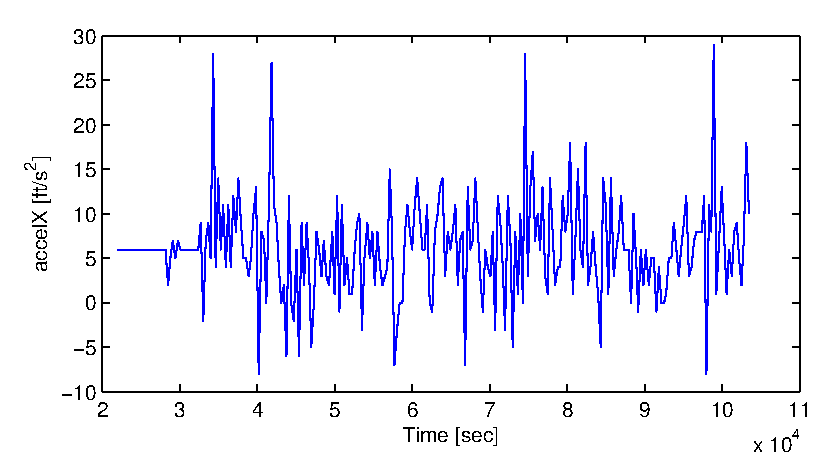
\includegraphics[width = 0.7\textwidth]{C:/Users/mufasa/Documents/Thesis/LaTex/figures/sampleOutput/Raw/accelX.eps}
\end{figure}
\begin{figure}[H]
	\centering
	\caption{accelY vs. Time}
		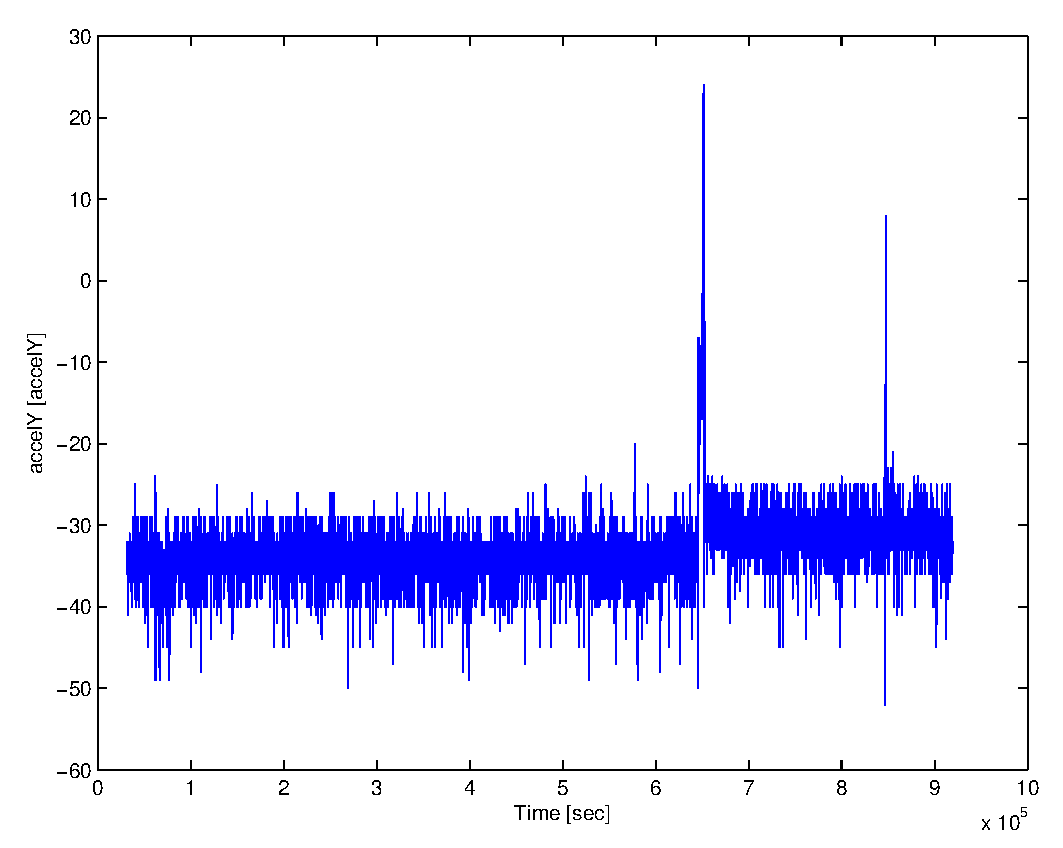
\includegraphics[width = 0.7\textwidth]{C:/Users/mufasa/Documents/Thesis/LaTex/figures/sampleOutput/Raw/accelY.eps}
\end{figure}
\begin{figure}[H]
	\centering
	\caption{accelZ vs. Time}
		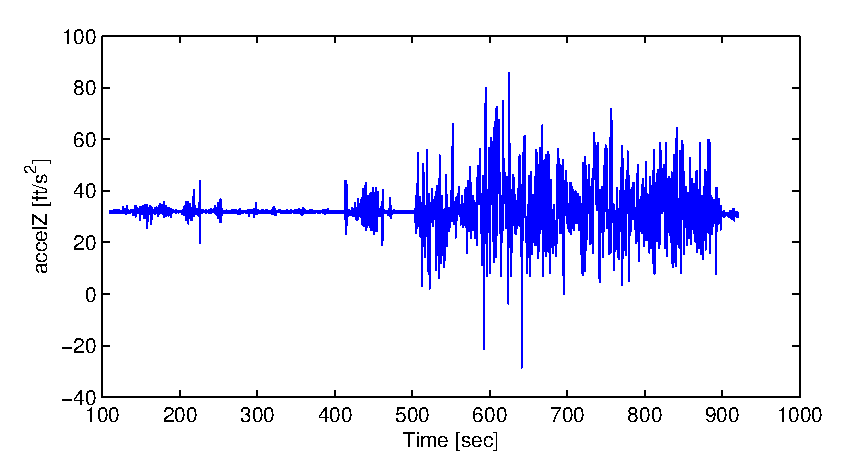
\includegraphics[width = 0.7\textwidth]{C:/Users/mufasa/Documents/Thesis/LaTex/figures/sampleOutput/Raw/accelZ.eps}
\end{figure}
\begin{figure}[H]
	\centering
	\caption{gyroX vs. Time}
		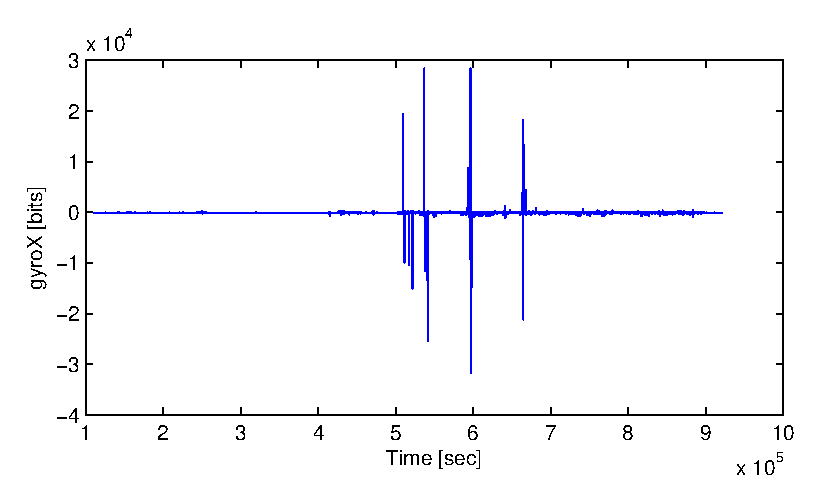
\includegraphics[width = 0.7\textwidth]{C:/Users/mufasa/Documents/Thesis/LaTex/figures/sampleOutput/Raw/gyroX.eps}
\end{figure}
\begin{figure}[H]
	\centering
	\caption{gyroY vs. Time}
		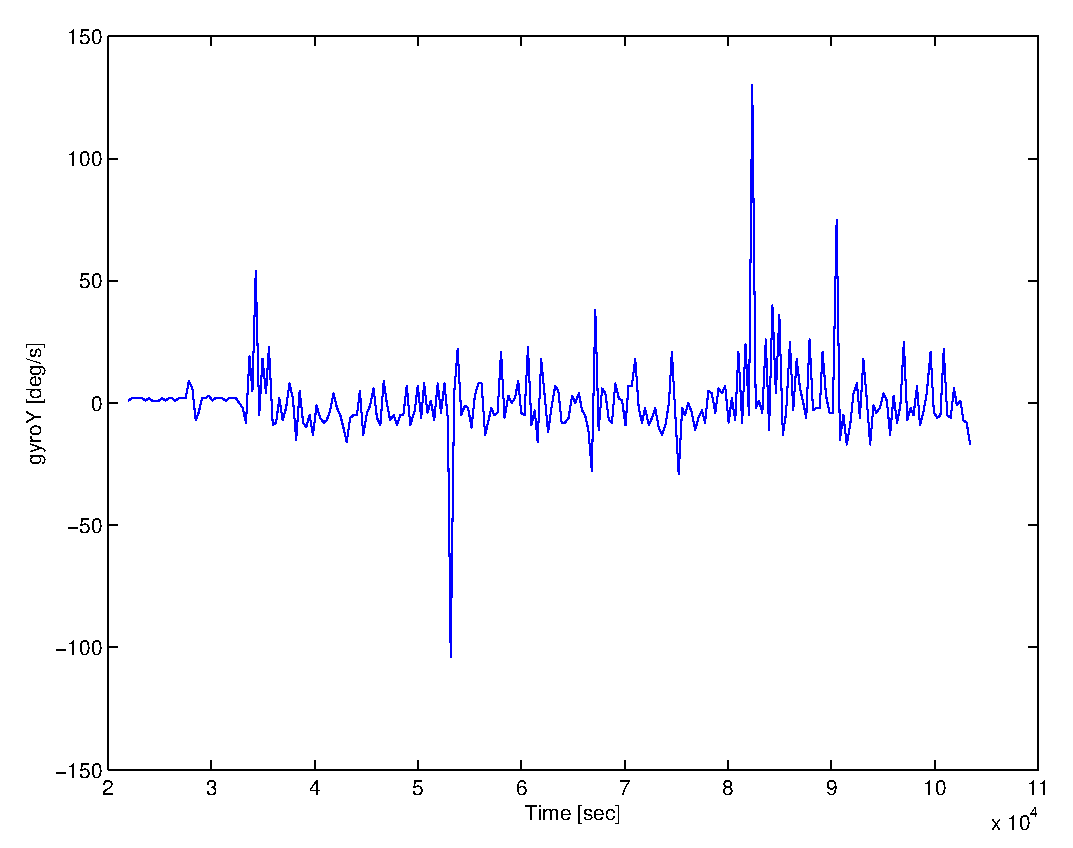
\includegraphics[width = 0.7\textwidth]{C:/Users/mufasa/Documents/Thesis/LaTex/figures/sampleOutput/Raw/gyroY.eps}
\end{figure}
\begin{figure}[H]
	\centering
	\caption{gyroZ vs. Time}
		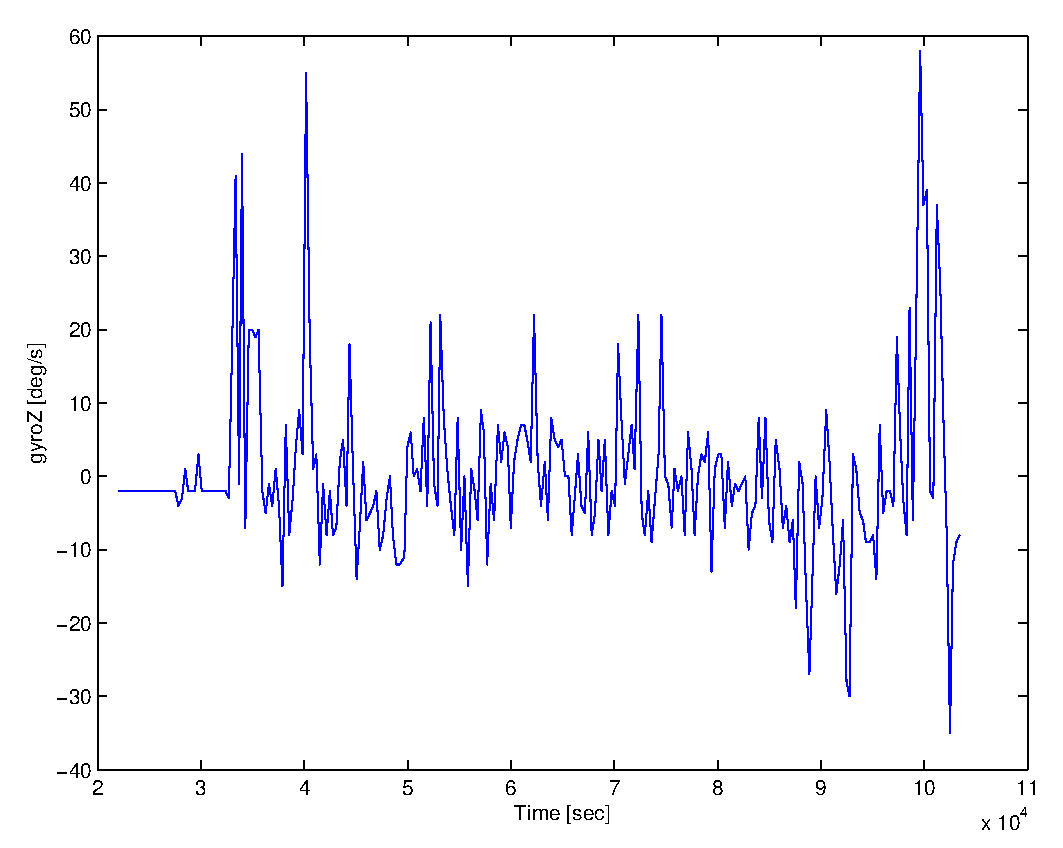
\includegraphics[width = 0.7\textwidth]{C:/Users/mufasa/Documents/Thesis/LaTex/figures/sampleOutput/Raw/gyroZ.eps}
\end{figure}
\begin{figure}[H]
	\centering
	\caption{magX vs. Time}
		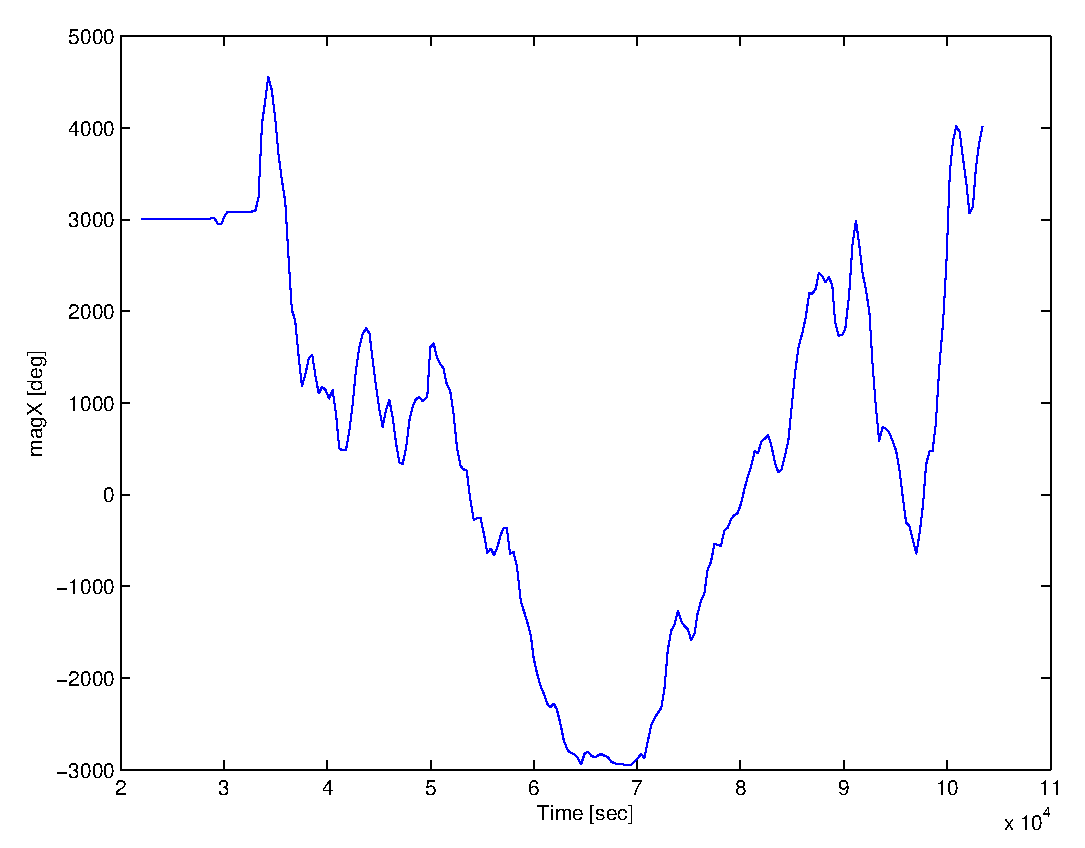
\includegraphics[width = 0.7\textwidth]{C:/Users/mufasa/Documents/Thesis/LaTex/figures/sampleOutput/Raw/magX.eps}
\end{figure}
\clearpage
\begin{figure}[H]
	\centering
	\caption{magY vs. Time}
		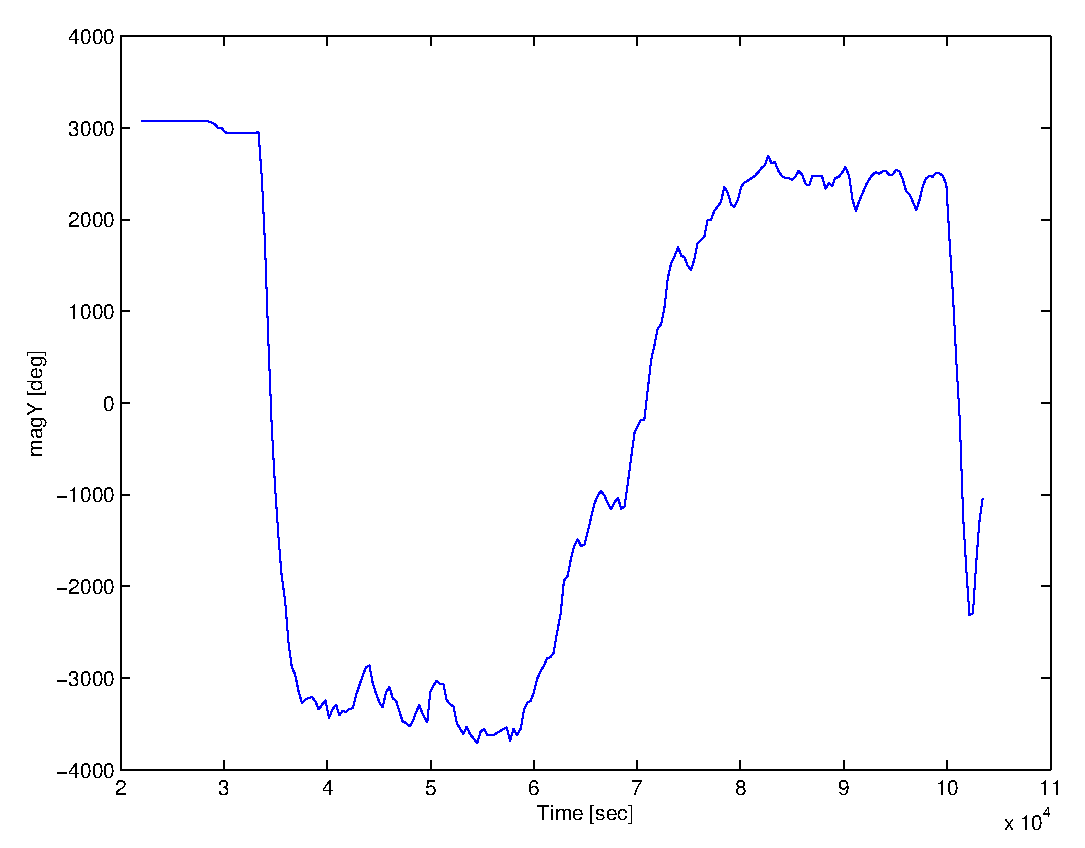
\includegraphics[width = 0.7\textwidth]{C:/Users/mufasa/Documents/Thesis/LaTex/figures/sampleOutput/Raw/magY.eps}
\end{figure}
\begin{figure}[H]
	\centering
	\caption{magZ vs. Time}
		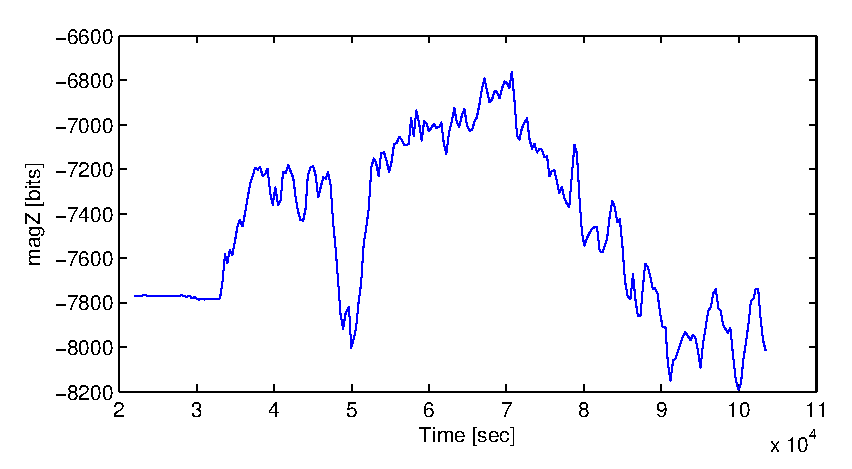
\includegraphics[width = 0.7\textwidth]{C:/Users/mufasa/Documents/Thesis/LaTex/figures/sampleOutput/Raw/magZ.eps}
\end{figure}
\begin{figure}[H]
	\centering
	\caption{hmcX vs. Time}
		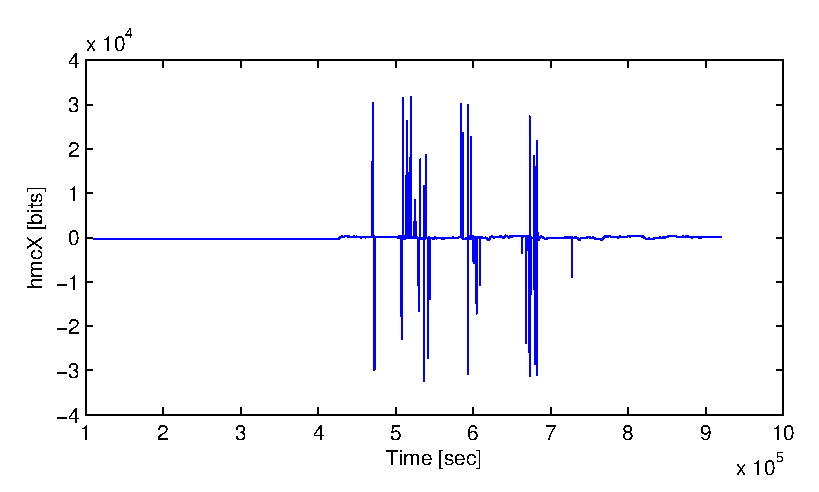
\includegraphics[width = 0.7\textwidth]{C:/Users/mufasa/Documents/Thesis/LaTex/figures/sampleOutput/Raw/hmcX.eps}
\end{figure}
\begin{figure}[H]
	\centering
	\caption{hmcZ vs. Time}
		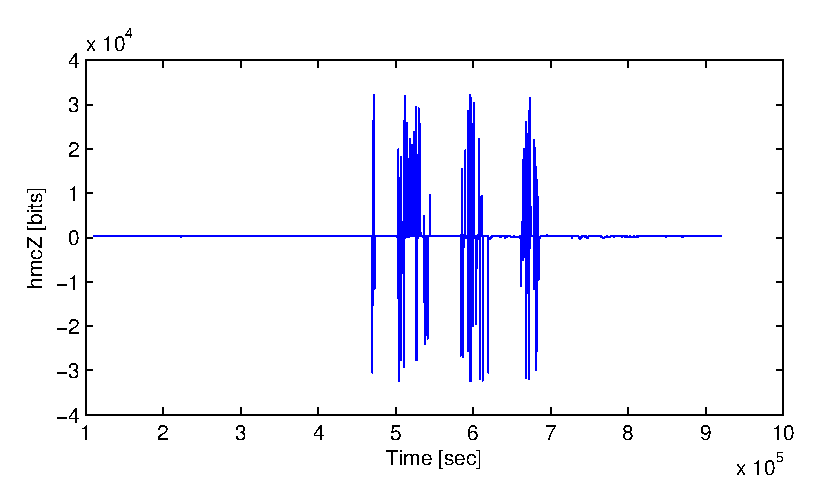
\includegraphics[width = 0.7\textwidth]{C:/Users/mufasa/Documents/Thesis/LaTex/figures/sampleOutput/Raw/hmcZ.eps}
\end{figure}
\begin{figure}[H]
	\centering
	\caption{hmcY vs. Time}
		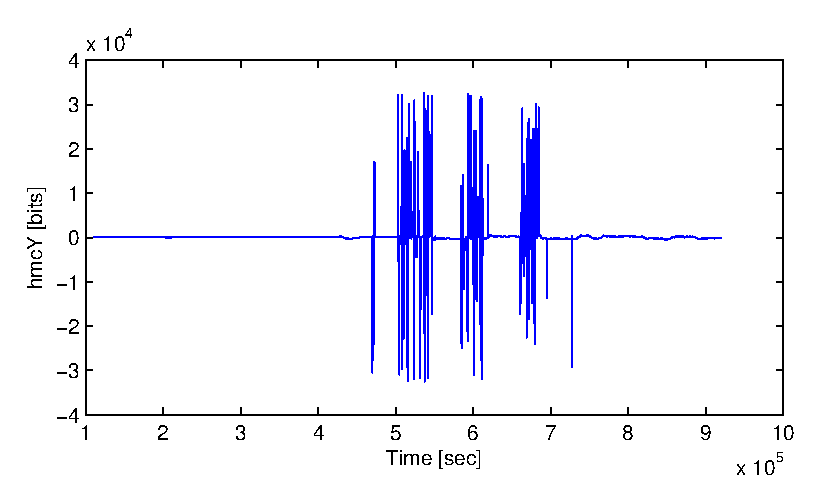
\includegraphics[width = 0.7\textwidth]{C:/Users/mufasa/Documents/Thesis/LaTex/figures/sampleOutput/Raw/hmcY.eps}
\end{figure}
\begin{figure}[H]
	\centering
	\caption{press0 vs. Time}
		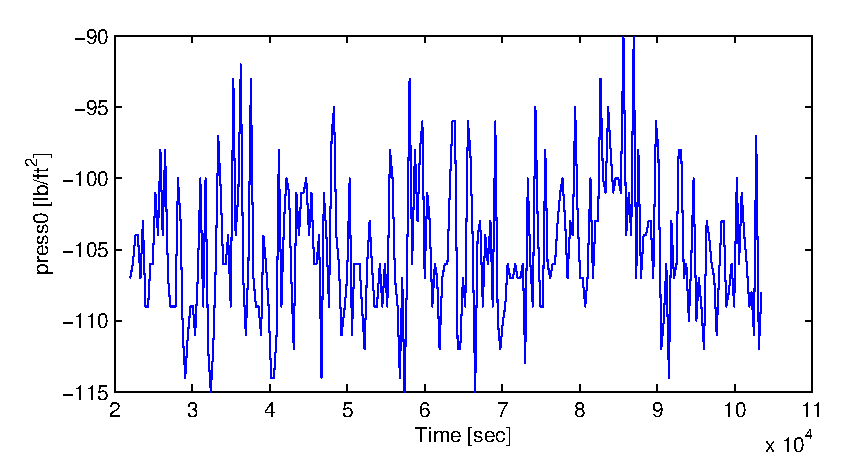
\includegraphics[width = 0.7\textwidth]{C:/Users/mufasa/Documents/Thesis/LaTex/figures/sampleOutput/Raw/press0.eps}
\end{figure}
\begin{figure}[H]
	\centering
	\caption{press1 vs. Time}
		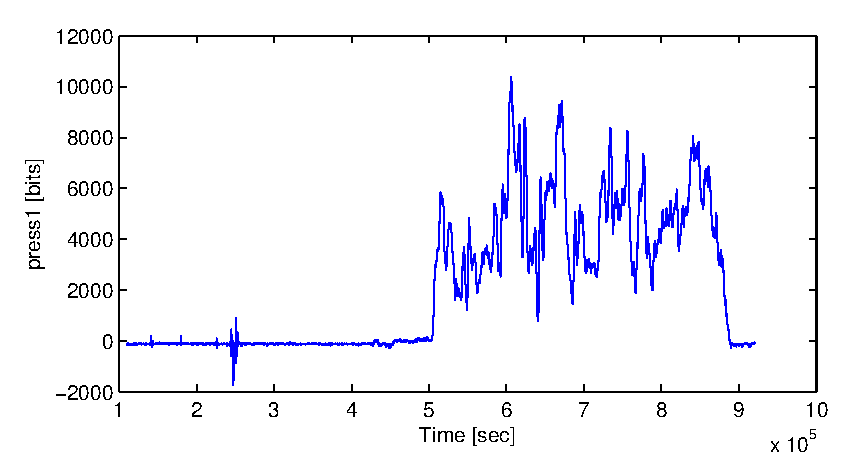
\includegraphics[width = 0.7\textwidth]{C:/Users/mufasa/Documents/Thesis/LaTex/figures/sampleOutput/Raw/press1.eps}
\end{figure}
\begin{figure}[H]
	\centering
	\caption{press2 vs. Time}
		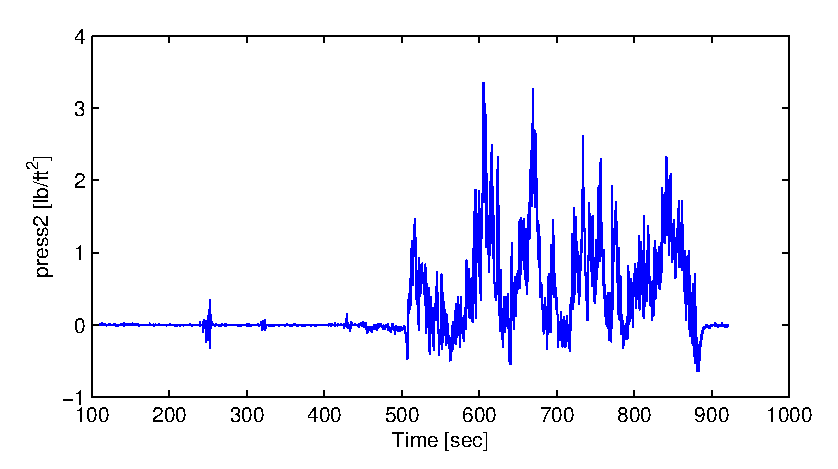
\includegraphics[width = 0.7\textwidth]{C:/Users/mufasa/Documents/Thesis/LaTex/figures/sampleOutput/Raw/press2.eps}
\end{figure}
\begin{figure}[H]
	\centering
	\caption{press3 vs. Time}
		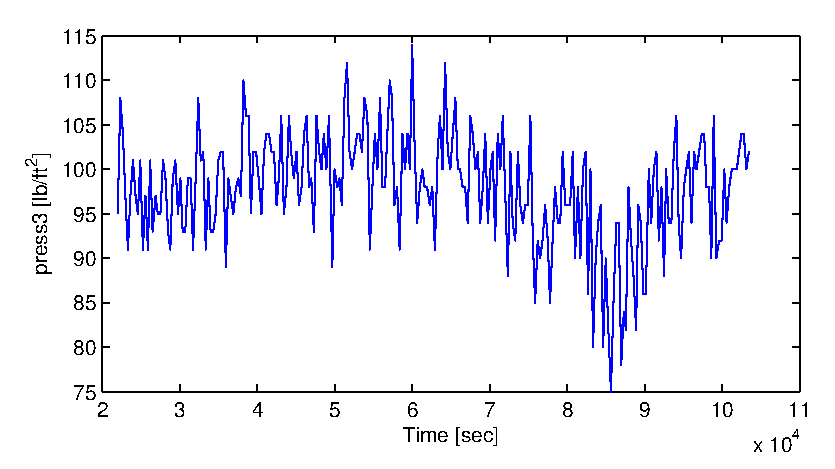
\includegraphics[width = 0.7\textwidth]{C:/Users/mufasa/Documents/Thesis/LaTex/figures/sampleOutput/Raw/press3.eps}
\end{figure}
\begin{figure}[H]
	\centering
	\caption{gpsLat vs. Time}
		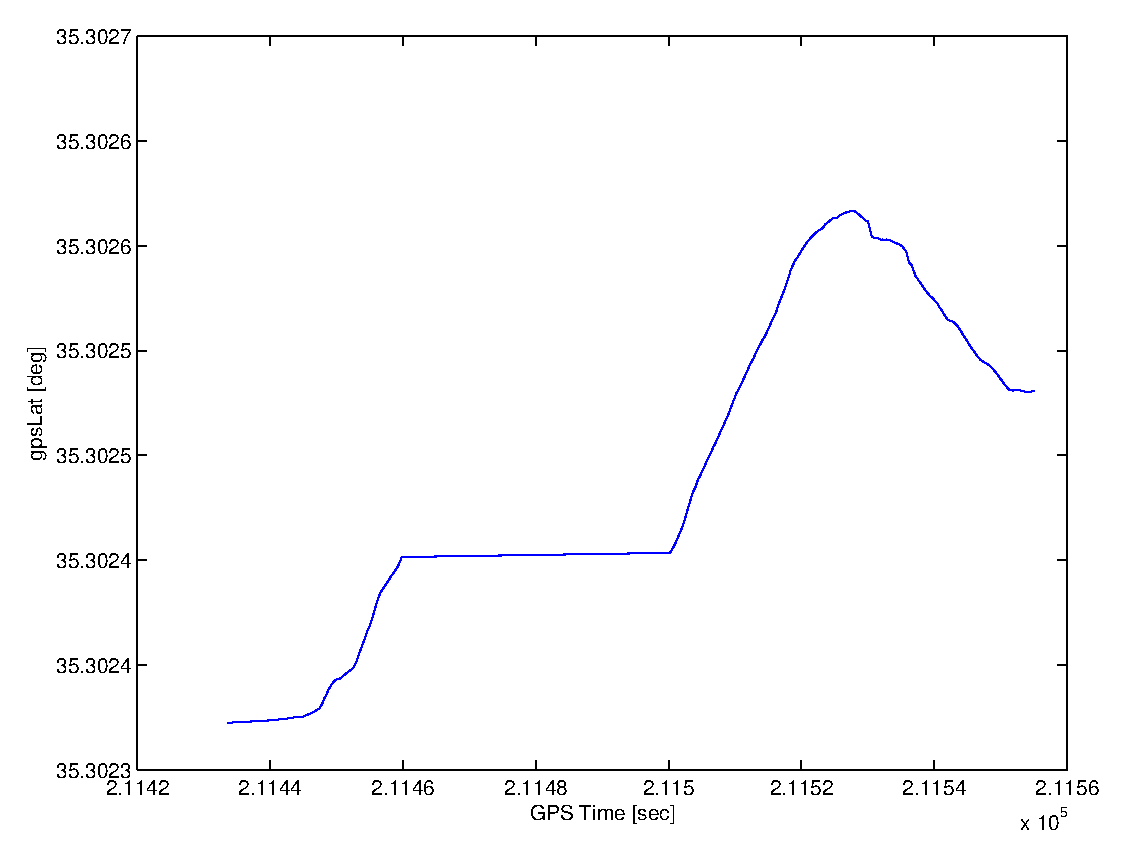
\includegraphics[width = 0.7\textwidth]{C:/Users/mufasa/Documents/Thesis/LaTex/figures/sampleOutput/Raw/gpsLat.eps}
\end{figure}
\begin{figure}[H]
	\centering
	\caption{gpsLong vs. Time}
		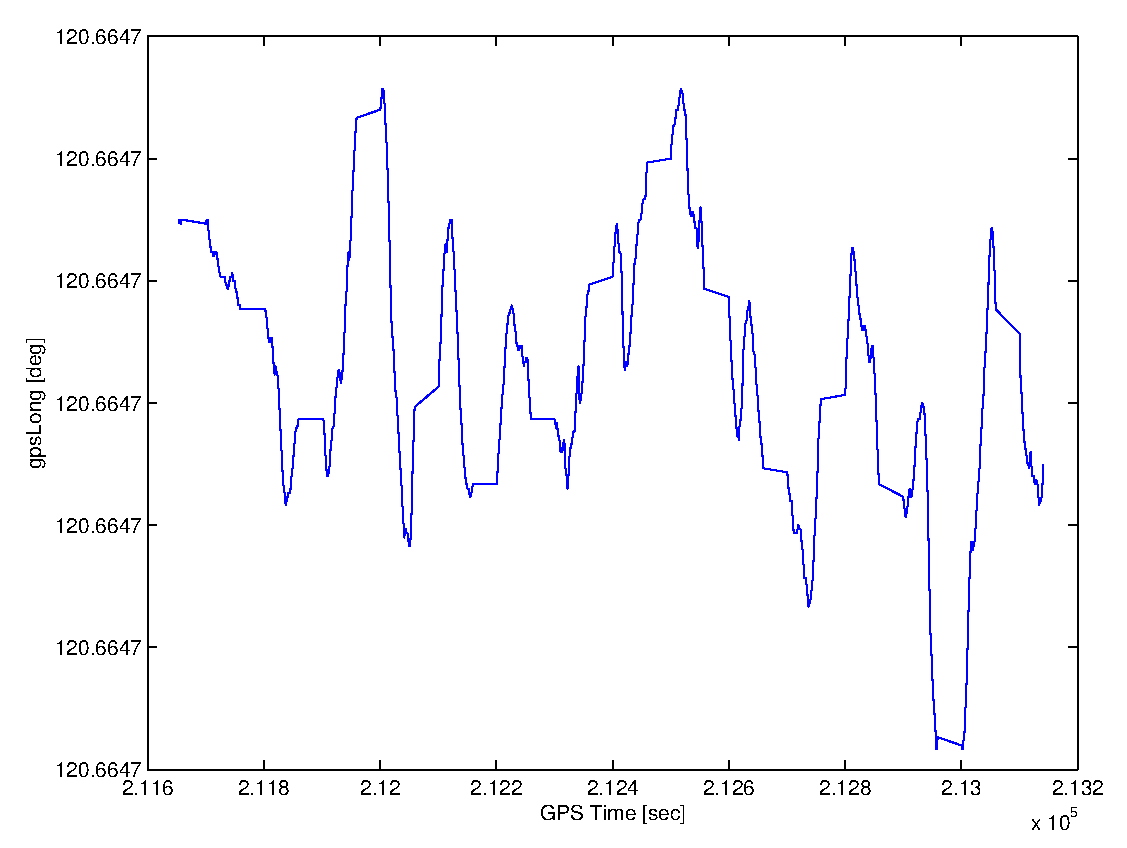
\includegraphics[width = 0.7\textwidth]{C:/Users/mufasa/Documents/Thesis/LaTex/figures/sampleOutput/Raw/gpsLong.eps}
\end{figure}
\begin{figure}[H]
	\centering
	\caption{gpsSpd vs. Time}
		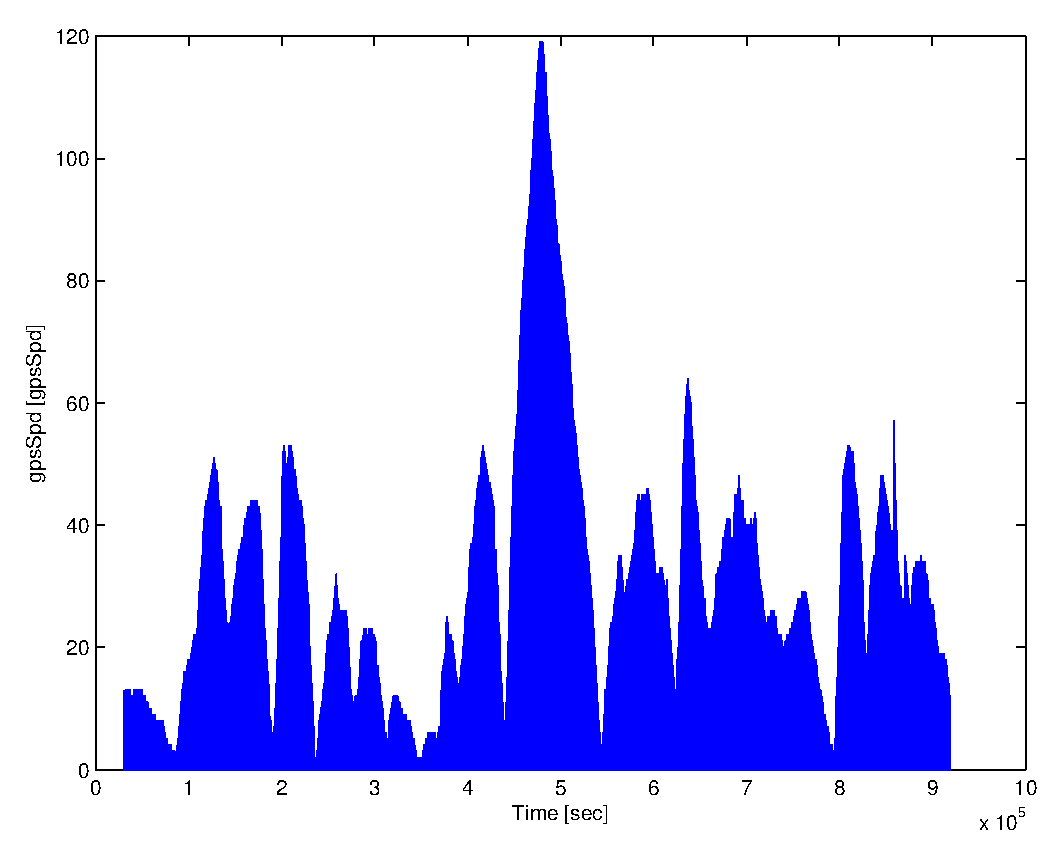
\includegraphics[width = 0.7\textwidth]{C:/Users/mufasa/Documents/Thesis/LaTex/figures/sampleOutput/Raw/gpsSpd.eps}
\end{figure}
\begin{figure}[H]
	\centering
	\caption{gpsCrs vs. Time}
		\includegraphics[width = 0.7\textwidth]{C:/Users/mufasa/Documents/Thesis/LaTex/figures/sampleOutput/Raw/gpsCrs.eps}
\end{figure}
\begin{figure}[H]
	\centering
	\caption{date vs. Time}
		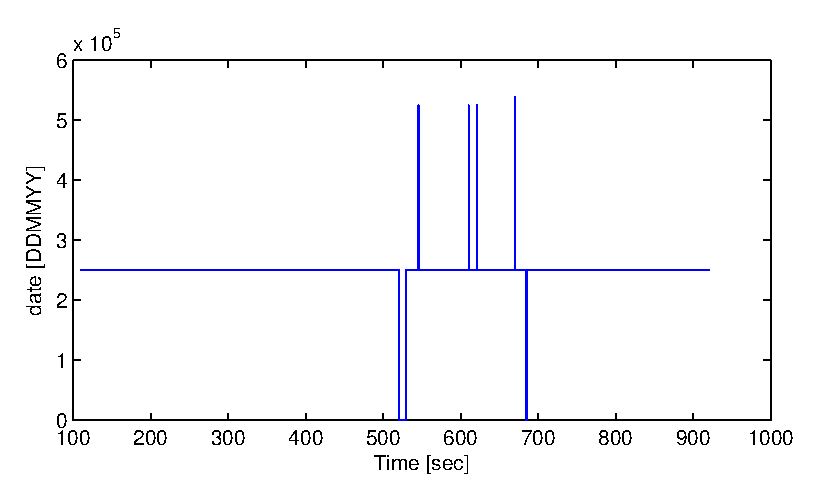
\includegraphics[width = 0.7\textwidth]{C:/Users/mufasa/Documents/Thesis/LaTex/figures/sampleOutput/Raw/date.eps}
\end{figure}
\begin{figure}[H]
	\centering
	\caption{CS vs. Time}
		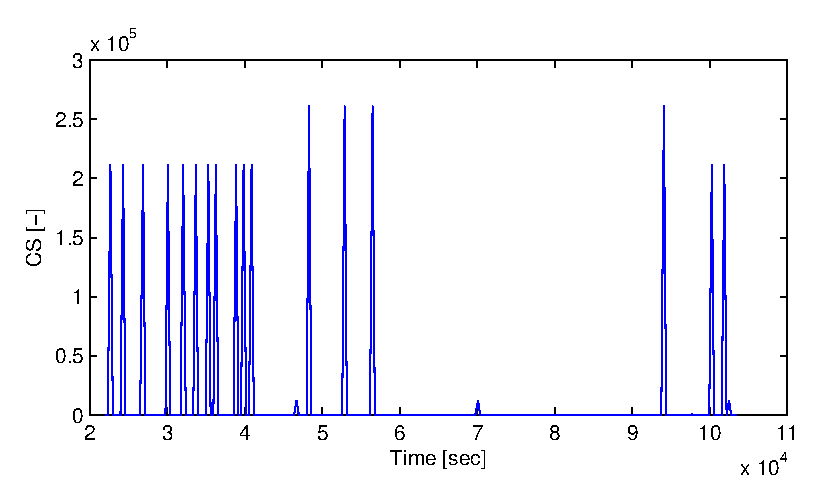
\includegraphics[width = 0.7\textwidth]{C:/Users/mufasa/Documents/Thesis/LaTex/figures/sampleOutput/Raw/CS.eps}
\end{figure}
\begin{figure}[H]
	\centering
	\caption{temperature vs. Time}
		\includegraphics[width = 0.7\textwidth]{C:/Users/mufasa/Documents/Thesis/LaTex/figures/sampleOutput/Raw/temperature.eps}
\end{figure}
\begin{figure}[H]
	\centering
	\caption{pwm0 vs. Time}
		\includegraphics[width = 0.7\textwidth]{C:/Users/mufasa/Documents/Thesis/LaTex/figures/sampleOutput/Raw/pwm0.eps}
\end{figure}
\begin{figure}[H]
	\centering
	\caption{pwm1 vs. Time}
		\includegraphics[width = 0.7\textwidth]{C:/Users/mufasa/Documents/Thesis/LaTex/figures/sampleOutput/Raw/pwm1.eps}
\end{figure}
\begin{figure}[H]
	\centering
	\caption{pwm2 vs. Time}
		\includegraphics[width = 0.7\textwidth]{C:/Users/mufasa/Documents/Thesis/LaTex/figures/sampleOutput/Raw/pwm2.eps}
\end{figure}
\begin{figure}[H]
	\centering
	\caption{pwm3 vs. Time}
		\includegraphics[width = 0.7\textwidth]{C:/Users/mufasa/Documents/Thesis/LaTex/figures/sampleOutput/Raw/pwm3.eps}
\end{figure}
\begin{figure}[H]
	\centering
	\caption{pwm4 vs. Time}
		\includegraphics[width = 0.7\textwidth]{C:/Users/mufasa/Documents/Thesis/LaTex/figures/sampleOutput/Raw/pwm4.eps}
\end{figure}
\begin{figure}[H]
	\centering
	\caption{pwm5 vs. Time}
		\includegraphics[width = 0.7\textwidth]{C:/Users/mufasa/Documents/Thesis/LaTex/figures/sampleOutput/Raw/pwm5.eps}
\end{figure}
\begin{figure}[H]
	\centering
	\caption{pwm6 vs. Time}
		\includegraphics[width = 0.7\textwidth]{C:/Users/mufasa/Documents/Thesis/LaTex/figures/sampleOutput/Raw/pwm6.eps}
\end{figure}
\begin{figure}[H]
	\centering
	\caption{pwm7 vs. Time}
		\includegraphics[width = 0.7\textwidth]{C:/Users/mufasa/Documents/Thesis/LaTex/figures/sampleOutput/Raw/pwm7.eps}
\end{figure}
\begin{figure}[H]
	\centering
	\caption{deltaT vs. Time}
		\includegraphics[width = 0.7\textwidth]{C:/Users/mufasa/Documents/Thesis/LaTex/figures/sampleOutput/Raw/deltaT.eps}
\end{figure}

%\section{Sample System Ouput - Raw Data}
\begin{figure}[H]
	\centering
	\caption{accelX vs. Time}
		\includegraphics[width = 0.7\textwidth]{C:/Users/mufasa/Documents/Thesis/LaTex/figures/sampleOutput/Raw/accelX.eps}
\end{figure}
\begin{figure}[H]
	\centering
	\caption{accelY vs. Time}
		\includegraphics[width = 0.7\textwidth]{C:/Users/mufasa/Documents/Thesis/LaTex/figures/sampleOutput/Raw/accelY.eps}
\end{figure}
\begin{figure}[H]
	\centering
	\caption{accelZ vs. Time}
		\includegraphics[width = 0.7\textwidth]{C:/Users/mufasa/Documents/Thesis/LaTex/figures/sampleOutput/Raw/accelZ.eps}
\end{figure}
\begin{figure}[H]
	\centering
	\caption{gyroX vs. Time}
		\includegraphics[width = 0.7\textwidth]{C:/Users/mufasa/Documents/Thesis/LaTex/figures/sampleOutput/Raw/gyroX.eps}
\end{figure}
\begin{figure}[H]
	\centering
	\caption{gyroY vs. Time}
		\includegraphics[width = 0.7\textwidth]{C:/Users/mufasa/Documents/Thesis/LaTex/figures/sampleOutput/Raw/gyroY.eps}
\end{figure}
\begin{figure}[H]
	\centering
	\caption{gyroZ vs. Time}
		\includegraphics[width = 0.7\textwidth]{C:/Users/mufasa/Documents/Thesis/LaTex/figures/sampleOutput/Raw/gyroZ.eps}
\end{figure}
\begin{figure}[H]
	\centering
	\caption{magX vs. Time}
		\includegraphics[width = 0.7\textwidth]{C:/Users/mufasa/Documents/Thesis/LaTex/figures/sampleOutput/Raw/magX.eps}
\end{figure}
\clearpage
\begin{figure}[H]
	\centering
	\caption{magY vs. Time}
		\includegraphics[width = 0.7\textwidth]{C:/Users/mufasa/Documents/Thesis/LaTex/figures/sampleOutput/Raw/magY.eps}
\end{figure}
\begin{figure}[H]
	\centering
	\caption{magZ vs. Time}
		\includegraphics[width = 0.7\textwidth]{C:/Users/mufasa/Documents/Thesis/LaTex/figures/sampleOutput/Raw/magZ.eps}
\end{figure}
\begin{figure}[H]
	\centering
	\caption{hmcX vs. Time}
		\includegraphics[width = 0.7\textwidth]{C:/Users/mufasa/Documents/Thesis/LaTex/figures/sampleOutput/Raw/hmcX.eps}
\end{figure}
\begin{figure}[H]
	\centering
	\caption{hmcZ vs. Time}
		\includegraphics[width = 0.7\textwidth]{C:/Users/mufasa/Documents/Thesis/LaTex/figures/sampleOutput/Raw/hmcZ.eps}
\end{figure}
\begin{figure}[H]
	\centering
	\caption{hmcY vs. Time}
		\includegraphics[width = 0.7\textwidth]{C:/Users/mufasa/Documents/Thesis/LaTex/figures/sampleOutput/Raw/hmcY.eps}
\end{figure}
\begin{figure}[H]
	\centering
	\caption{press0 vs. Time}
		\includegraphics[width = 0.7\textwidth]{C:/Users/mufasa/Documents/Thesis/LaTex/figures/sampleOutput/Raw/press0.eps}
\end{figure}
\begin{figure}[H]
	\centering
	\caption{press1 vs. Time}
		\includegraphics[width = 0.7\textwidth]{C:/Users/mufasa/Documents/Thesis/LaTex/figures/sampleOutput/Raw/press1.eps}
\end{figure}
\begin{figure}[H]
	\centering
	\caption{press2 vs. Time}
		\includegraphics[width = 0.7\textwidth]{C:/Users/mufasa/Documents/Thesis/LaTex/figures/sampleOutput/Raw/press2.eps}
\end{figure}
\begin{figure}[H]
	\centering
	\caption{press3 vs. Time}
		\includegraphics[width = 0.7\textwidth]{C:/Users/mufasa/Documents/Thesis/LaTex/figures/sampleOutput/Raw/press3.eps}
\end{figure}
\begin{figure}[H]
	\centering
	\caption{gpsLat vs. Time}
		\includegraphics[width = 0.7\textwidth]{C:/Users/mufasa/Documents/Thesis/LaTex/figures/sampleOutput/Raw/gpsLat.eps}
\end{figure}
\begin{figure}[H]
	\centering
	\caption{gpsLong vs. Time}
		\includegraphics[width = 0.7\textwidth]{C:/Users/mufasa/Documents/Thesis/LaTex/figures/sampleOutput/Raw/gpsLong.eps}
\end{figure}
\begin{figure}[H]
	\centering
	\caption{gpsSpd vs. Time}
		\includegraphics[width = 0.7\textwidth]{C:/Users/mufasa/Documents/Thesis/LaTex/figures/sampleOutput/Raw/gpsSpd.eps}
\end{figure}
\begin{figure}[H]
	\centering
	\caption{gpsCrs vs. Time}
		\includegraphics[width = 0.7\textwidth]{C:/Users/mufasa/Documents/Thesis/LaTex/figures/sampleOutput/Raw/gpsCrs.eps}
\end{figure}
\begin{figure}[H]
	\centering
	\caption{date vs. Time}
		\includegraphics[width = 0.7\textwidth]{C:/Users/mufasa/Documents/Thesis/LaTex/figures/sampleOutput/Raw/date.eps}
\end{figure}
\begin{figure}[H]
	\centering
	\caption{CS vs. Time}
		\includegraphics[width = 0.7\textwidth]{C:/Users/mufasa/Documents/Thesis/LaTex/figures/sampleOutput/Raw/CS.eps}
\end{figure}
\begin{figure}[H]
	\centering
	\caption{temperature vs. Time}
		\includegraphics[width = 0.7\textwidth]{C:/Users/mufasa/Documents/Thesis/LaTex/figures/sampleOutput/Raw/temperature.eps}
\end{figure}
\begin{figure}[H]
	\centering
	\caption{pwm0 vs. Time}
		\includegraphics[width = 0.7\textwidth]{C:/Users/mufasa/Documents/Thesis/LaTex/figures/sampleOutput/Raw/pwm0.eps}
\end{figure}
\begin{figure}[H]
	\centering
	\caption{pwm1 vs. Time}
		\includegraphics[width = 0.7\textwidth]{C:/Users/mufasa/Documents/Thesis/LaTex/figures/sampleOutput/Raw/pwm1.eps}
\end{figure}
\begin{figure}[H]
	\centering
	\caption{pwm2 vs. Time}
		\includegraphics[width = 0.7\textwidth]{C:/Users/mufasa/Documents/Thesis/LaTex/figures/sampleOutput/Raw/pwm2.eps}
\end{figure}
\begin{figure}[H]
	\centering
	\caption{pwm3 vs. Time}
		\includegraphics[width = 0.7\textwidth]{C:/Users/mufasa/Documents/Thesis/LaTex/figures/sampleOutput/Raw/pwm3.eps}
\end{figure}
\begin{figure}[H]
	\centering
	\caption{pwm4 vs. Time}
		\includegraphics[width = 0.7\textwidth]{C:/Users/mufasa/Documents/Thesis/LaTex/figures/sampleOutput/Raw/pwm4.eps}
\end{figure}
\begin{figure}[H]
	\centering
	\caption{pwm5 vs. Time}
		\includegraphics[width = 0.7\textwidth]{C:/Users/mufasa/Documents/Thesis/LaTex/figures/sampleOutput/Raw/pwm5.eps}
\end{figure}
\begin{figure}[H]
	\centering
	\caption{pwm6 vs. Time}
		\includegraphics[width = 0.7\textwidth]{C:/Users/mufasa/Documents/Thesis/LaTex/figures/sampleOutput/Raw/pwm6.eps}
\end{figure}
\begin{figure}[H]
	\centering
	\caption{pwm7 vs. Time}
		\includegraphics[width = 0.7\textwidth]{C:/Users/mufasa/Documents/Thesis/LaTex/figures/sampleOutput/Raw/pwm7.eps}
\end{figure}
\begin{figure}[H]
	\centering
	\caption{deltaT vs. Time}
		\includegraphics[width = 0.7\textwidth]{C:/Users/mufasa/Documents/Thesis/LaTex/figures/sampleOutput/Raw/deltaT.eps}
\end{figure}

%\section{Sample System Ouput - Raw Data}
\begin{figure}[H]
	\centering
	\caption{accelX vs. Time}
		\includegraphics[width = 0.7\textwidth]{C:/Users/mufasa/Documents/Thesis/LaTex/figures/sampleOutput/Raw/accelX.eps}
\end{figure}
\begin{figure}[H]
	\centering
	\caption{accelY vs. Time}
		\includegraphics[width = 0.7\textwidth]{C:/Users/mufasa/Documents/Thesis/LaTex/figures/sampleOutput/Raw/accelY.eps}
\end{figure}
\begin{figure}[H]
	\centering
	\caption{accelZ vs. Time}
		\includegraphics[width = 0.7\textwidth]{C:/Users/mufasa/Documents/Thesis/LaTex/figures/sampleOutput/Raw/accelZ.eps}
\end{figure}
\begin{figure}[H]
	\centering
	\caption{gyroX vs. Time}
		\includegraphics[width = 0.7\textwidth]{C:/Users/mufasa/Documents/Thesis/LaTex/figures/sampleOutput/Raw/gyroX.eps}
\end{figure}
\begin{figure}[H]
	\centering
	\caption{gyroY vs. Time}
		\includegraphics[width = 0.7\textwidth]{C:/Users/mufasa/Documents/Thesis/LaTex/figures/sampleOutput/Raw/gyroY.eps}
\end{figure}
\begin{figure}[H]
	\centering
	\caption{gyroZ vs. Time}
		\includegraphics[width = 0.7\textwidth]{C:/Users/mufasa/Documents/Thesis/LaTex/figures/sampleOutput/Raw/gyroZ.eps}
\end{figure}
\begin{figure}[H]
	\centering
	\caption{magX vs. Time}
		\includegraphics[width = 0.7\textwidth]{C:/Users/mufasa/Documents/Thesis/LaTex/figures/sampleOutput/Raw/magX.eps}
\end{figure}
\clearpage
\begin{figure}[H]
	\centering
	\caption{magY vs. Time}
		\includegraphics[width = 0.7\textwidth]{C:/Users/mufasa/Documents/Thesis/LaTex/figures/sampleOutput/Raw/magY.eps}
\end{figure}
\begin{figure}[H]
	\centering
	\caption{magZ vs. Time}
		\includegraphics[width = 0.7\textwidth]{C:/Users/mufasa/Documents/Thesis/LaTex/figures/sampleOutput/Raw/magZ.eps}
\end{figure}
\begin{figure}[H]
	\centering
	\caption{hmcX vs. Time}
		\includegraphics[width = 0.7\textwidth]{C:/Users/mufasa/Documents/Thesis/LaTex/figures/sampleOutput/Raw/hmcX.eps}
\end{figure}
\begin{figure}[H]
	\centering
	\caption{hmcZ vs. Time}
		\includegraphics[width = 0.7\textwidth]{C:/Users/mufasa/Documents/Thesis/LaTex/figures/sampleOutput/Raw/hmcZ.eps}
\end{figure}
\begin{figure}[H]
	\centering
	\caption{hmcY vs. Time}
		\includegraphics[width = 0.7\textwidth]{C:/Users/mufasa/Documents/Thesis/LaTex/figures/sampleOutput/Raw/hmcY.eps}
\end{figure}
\begin{figure}[H]
	\centering
	\caption{press0 vs. Time}
		\includegraphics[width = 0.7\textwidth]{C:/Users/mufasa/Documents/Thesis/LaTex/figures/sampleOutput/Raw/press0.eps}
\end{figure}
\begin{figure}[H]
	\centering
	\caption{press1 vs. Time}
		\includegraphics[width = 0.7\textwidth]{C:/Users/mufasa/Documents/Thesis/LaTex/figures/sampleOutput/Raw/press1.eps}
\end{figure}
\begin{figure}[H]
	\centering
	\caption{press2 vs. Time}
		\includegraphics[width = 0.7\textwidth]{C:/Users/mufasa/Documents/Thesis/LaTex/figures/sampleOutput/Raw/press2.eps}
\end{figure}
\begin{figure}[H]
	\centering
	\caption{press3 vs. Time}
		\includegraphics[width = 0.7\textwidth]{C:/Users/mufasa/Documents/Thesis/LaTex/figures/sampleOutput/Raw/press3.eps}
\end{figure}
\begin{figure}[H]
	\centering
	\caption{gpsLat vs. Time}
		\includegraphics[width = 0.7\textwidth]{C:/Users/mufasa/Documents/Thesis/LaTex/figures/sampleOutput/Raw/gpsLat.eps}
\end{figure}
\begin{figure}[H]
	\centering
	\caption{gpsLong vs. Time}
		\includegraphics[width = 0.7\textwidth]{C:/Users/mufasa/Documents/Thesis/LaTex/figures/sampleOutput/Raw/gpsLong.eps}
\end{figure}
\begin{figure}[H]
	\centering
	\caption{gpsSpd vs. Time}
		\includegraphics[width = 0.7\textwidth]{C:/Users/mufasa/Documents/Thesis/LaTex/figures/sampleOutput/Raw/gpsSpd.eps}
\end{figure}
\begin{figure}[H]
	\centering
	\caption{gpsCrs vs. Time}
		\includegraphics[width = 0.7\textwidth]{C:/Users/mufasa/Documents/Thesis/LaTex/figures/sampleOutput/Raw/gpsCrs.eps}
\end{figure}
\begin{figure}[H]
	\centering
	\caption{date vs. Time}
		\includegraphics[width = 0.7\textwidth]{C:/Users/mufasa/Documents/Thesis/LaTex/figures/sampleOutput/Raw/date.eps}
\end{figure}
\begin{figure}[H]
	\centering
	\caption{CS vs. Time}
		\includegraphics[width = 0.7\textwidth]{C:/Users/mufasa/Documents/Thesis/LaTex/figures/sampleOutput/Raw/CS.eps}
\end{figure}
\begin{figure}[H]
	\centering
	\caption{temperature vs. Time}
		\includegraphics[width = 0.7\textwidth]{C:/Users/mufasa/Documents/Thesis/LaTex/figures/sampleOutput/Raw/temperature.eps}
\end{figure}
\begin{figure}[H]
	\centering
	\caption{pwm0 vs. Time}
		\includegraphics[width = 0.7\textwidth]{C:/Users/mufasa/Documents/Thesis/LaTex/figures/sampleOutput/Raw/pwm0.eps}
\end{figure}
\begin{figure}[H]
	\centering
	\caption{pwm1 vs. Time}
		\includegraphics[width = 0.7\textwidth]{C:/Users/mufasa/Documents/Thesis/LaTex/figures/sampleOutput/Raw/pwm1.eps}
\end{figure}
\begin{figure}[H]
	\centering
	\caption{pwm2 vs. Time}
		\includegraphics[width = 0.7\textwidth]{C:/Users/mufasa/Documents/Thesis/LaTex/figures/sampleOutput/Raw/pwm2.eps}
\end{figure}
\begin{figure}[H]
	\centering
	\caption{pwm3 vs. Time}
		\includegraphics[width = 0.7\textwidth]{C:/Users/mufasa/Documents/Thesis/LaTex/figures/sampleOutput/Raw/pwm3.eps}
\end{figure}
\begin{figure}[H]
	\centering
	\caption{pwm4 vs. Time}
		\includegraphics[width = 0.7\textwidth]{C:/Users/mufasa/Documents/Thesis/LaTex/figures/sampleOutput/Raw/pwm4.eps}
\end{figure}
\begin{figure}[H]
	\centering
	\caption{pwm5 vs. Time}
		\includegraphics[width = 0.7\textwidth]{C:/Users/mufasa/Documents/Thesis/LaTex/figures/sampleOutput/Raw/pwm5.eps}
\end{figure}
\begin{figure}[H]
	\centering
	\caption{pwm6 vs. Time}
		\includegraphics[width = 0.7\textwidth]{C:/Users/mufasa/Documents/Thesis/LaTex/figures/sampleOutput/Raw/pwm6.eps}
\end{figure}
\begin{figure}[H]
	\centering
	\caption{pwm7 vs. Time}
		\includegraphics[width = 0.7\textwidth]{C:/Users/mufasa/Documents/Thesis/LaTex/figures/sampleOutput/Raw/pwm7.eps}
\end{figure}
\begin{figure}[H]
	\centering
	\caption{deltaT vs. Time}
		\includegraphics[width = 0.7\textwidth]{C:/Users/mufasa/Documents/Thesis/LaTex/figures/sampleOutput/Raw/deltaT.eps}
\end{figure}

%\section{Sample System Ouput - Raw Data}
\begin{figure}[H]
	\centering
	\caption{accelX vs. Time}
		\includegraphics[width = 0.7\textwidth]{C:/Users/mufasa/Documents/Thesis/LaTex/figures/sampleOutput/Raw/accelX.eps}
\end{figure}
\begin{figure}[H]
	\centering
	\caption{accelY vs. Time}
		\includegraphics[width = 0.7\textwidth]{C:/Users/mufasa/Documents/Thesis/LaTex/figures/sampleOutput/Raw/accelY.eps}
\end{figure}
\begin{figure}[H]
	\centering
	\caption{accelZ vs. Time}
		\includegraphics[width = 0.7\textwidth]{C:/Users/mufasa/Documents/Thesis/LaTex/figures/sampleOutput/Raw/accelZ.eps}
\end{figure}
\begin{figure}[H]
	\centering
	\caption{gyroX vs. Time}
		\includegraphics[width = 0.7\textwidth]{C:/Users/mufasa/Documents/Thesis/LaTex/figures/sampleOutput/Raw/gyroX.eps}
\end{figure}
\begin{figure}[H]
	\centering
	\caption{gyroY vs. Time}
		\includegraphics[width = 0.7\textwidth]{C:/Users/mufasa/Documents/Thesis/LaTex/figures/sampleOutput/Raw/gyroY.eps}
\end{figure}
\begin{figure}[H]
	\centering
	\caption{gyroZ vs. Time}
		\includegraphics[width = 0.7\textwidth]{C:/Users/mufasa/Documents/Thesis/LaTex/figures/sampleOutput/Raw/gyroZ.eps}
\end{figure}
\begin{figure}[H]
	\centering
	\caption{magX vs. Time}
		\includegraphics[width = 0.7\textwidth]{C:/Users/mufasa/Documents/Thesis/LaTex/figures/sampleOutput/Raw/magX.eps}
\end{figure}
\clearpage
\begin{figure}[H]
	\centering
	\caption{magY vs. Time}
		\includegraphics[width = 0.7\textwidth]{C:/Users/mufasa/Documents/Thesis/LaTex/figures/sampleOutput/Raw/magY.eps}
\end{figure}
\begin{figure}[H]
	\centering
	\caption{magZ vs. Time}
		\includegraphics[width = 0.7\textwidth]{C:/Users/mufasa/Documents/Thesis/LaTex/figures/sampleOutput/Raw/magZ.eps}
\end{figure}
\begin{figure}[H]
	\centering
	\caption{hmcX vs. Time}
		\includegraphics[width = 0.7\textwidth]{C:/Users/mufasa/Documents/Thesis/LaTex/figures/sampleOutput/Raw/hmcX.eps}
\end{figure}
\begin{figure}[H]
	\centering
	\caption{hmcZ vs. Time}
		\includegraphics[width = 0.7\textwidth]{C:/Users/mufasa/Documents/Thesis/LaTex/figures/sampleOutput/Raw/hmcZ.eps}
\end{figure}
\begin{figure}[H]
	\centering
	\caption{hmcY vs. Time}
		\includegraphics[width = 0.7\textwidth]{C:/Users/mufasa/Documents/Thesis/LaTex/figures/sampleOutput/Raw/hmcY.eps}
\end{figure}
\begin{figure}[H]
	\centering
	\caption{press0 vs. Time}
		\includegraphics[width = 0.7\textwidth]{C:/Users/mufasa/Documents/Thesis/LaTex/figures/sampleOutput/Raw/press0.eps}
\end{figure}
\begin{figure}[H]
	\centering
	\caption{press1 vs. Time}
		\includegraphics[width = 0.7\textwidth]{C:/Users/mufasa/Documents/Thesis/LaTex/figures/sampleOutput/Raw/press1.eps}
\end{figure}
\begin{figure}[H]
	\centering
	\caption{press2 vs. Time}
		\includegraphics[width = 0.7\textwidth]{C:/Users/mufasa/Documents/Thesis/LaTex/figures/sampleOutput/Raw/press2.eps}
\end{figure}
\begin{figure}[H]
	\centering
	\caption{press3 vs. Time}
		\includegraphics[width = 0.7\textwidth]{C:/Users/mufasa/Documents/Thesis/LaTex/figures/sampleOutput/Raw/press3.eps}
\end{figure}
\begin{figure}[H]
	\centering
	\caption{gpsLat vs. Time}
		\includegraphics[width = 0.7\textwidth]{C:/Users/mufasa/Documents/Thesis/LaTex/figures/sampleOutput/Raw/gpsLat.eps}
\end{figure}
\begin{figure}[H]
	\centering
	\caption{gpsLong vs. Time}
		\includegraphics[width = 0.7\textwidth]{C:/Users/mufasa/Documents/Thesis/LaTex/figures/sampleOutput/Raw/gpsLong.eps}
\end{figure}
\begin{figure}[H]
	\centering
	\caption{gpsSpd vs. Time}
		\includegraphics[width = 0.7\textwidth]{C:/Users/mufasa/Documents/Thesis/LaTex/figures/sampleOutput/Raw/gpsSpd.eps}
\end{figure}
\begin{figure}[H]
	\centering
	\caption{gpsCrs vs. Time}
		\includegraphics[width = 0.7\textwidth]{C:/Users/mufasa/Documents/Thesis/LaTex/figures/sampleOutput/Raw/gpsCrs.eps}
\end{figure}
\begin{figure}[H]
	\centering
	\caption{date vs. Time}
		\includegraphics[width = 0.7\textwidth]{C:/Users/mufasa/Documents/Thesis/LaTex/figures/sampleOutput/Raw/date.eps}
\end{figure}
\begin{figure}[H]
	\centering
	\caption{CS vs. Time}
		\includegraphics[width = 0.7\textwidth]{C:/Users/mufasa/Documents/Thesis/LaTex/figures/sampleOutput/Raw/CS.eps}
\end{figure}
\begin{figure}[H]
	\centering
	\caption{temperature vs. Time}
		\includegraphics[width = 0.7\textwidth]{C:/Users/mufasa/Documents/Thesis/LaTex/figures/sampleOutput/Raw/temperature.eps}
\end{figure}
\begin{figure}[H]
	\centering
	\caption{pwm0 vs. Time}
		\includegraphics[width = 0.7\textwidth]{C:/Users/mufasa/Documents/Thesis/LaTex/figures/sampleOutput/Raw/pwm0.eps}
\end{figure}
\begin{figure}[H]
	\centering
	\caption{pwm1 vs. Time}
		\includegraphics[width = 0.7\textwidth]{C:/Users/mufasa/Documents/Thesis/LaTex/figures/sampleOutput/Raw/pwm1.eps}
\end{figure}
\begin{figure}[H]
	\centering
	\caption{pwm2 vs. Time}
		\includegraphics[width = 0.7\textwidth]{C:/Users/mufasa/Documents/Thesis/LaTex/figures/sampleOutput/Raw/pwm2.eps}
\end{figure}
\begin{figure}[H]
	\centering
	\caption{pwm3 vs. Time}
		\includegraphics[width = 0.7\textwidth]{C:/Users/mufasa/Documents/Thesis/LaTex/figures/sampleOutput/Raw/pwm3.eps}
\end{figure}
\begin{figure}[H]
	\centering
	\caption{pwm4 vs. Time}
		\includegraphics[width = 0.7\textwidth]{C:/Users/mufasa/Documents/Thesis/LaTex/figures/sampleOutput/Raw/pwm4.eps}
\end{figure}
\begin{figure}[H]
	\centering
	\caption{pwm5 vs. Time}
		\includegraphics[width = 0.7\textwidth]{C:/Users/mufasa/Documents/Thesis/LaTex/figures/sampleOutput/Raw/pwm5.eps}
\end{figure}
\begin{figure}[H]
	\centering
	\caption{pwm6 vs. Time}
		\includegraphics[width = 0.7\textwidth]{C:/Users/mufasa/Documents/Thesis/LaTex/figures/sampleOutput/Raw/pwm6.eps}
\end{figure}
\begin{figure}[H]
	\centering
	\caption{pwm7 vs. Time}
		\includegraphics[width = 0.7\textwidth]{C:/Users/mufasa/Documents/Thesis/LaTex/figures/sampleOutput/Raw/pwm7.eps}
\end{figure}
\begin{figure}[H]
	\centering
	\caption{deltaT vs. Time}
		\includegraphics[width = 0.7\textwidth]{C:/Users/mufasa/Documents/Thesis/LaTex/figures/sampleOutput/Raw/deltaT.eps}
\end{figure}

\chapter{Sample System Ouput}
This appendix contains graphs representing typical outputs from the data acquisition system, shown in strip chart format.
\section{Sample System Ouput - Raw Data}
\begin{figure}[H]
	\centering
	\caption{accelX vs. Time}
		\includegraphics[width = 0.7\textwidth]{C:/Users/mufasa/Documents/Thesis/LaTex/figures/sampleOutput/Raw/accelX.eps}
\end{figure}
\begin{figure}[H]
	\centering
	\caption{accelY vs. Time}
		\includegraphics[width = 0.7\textwidth]{C:/Users/mufasa/Documents/Thesis/LaTex/figures/sampleOutput/Raw/accelY.eps}
\end{figure}
\begin{figure}[H]
	\centering
	\caption{accelZ vs. Time}
		\includegraphics[width = 0.7\textwidth]{C:/Users/mufasa/Documents/Thesis/LaTex/figures/sampleOutput/Raw/accelZ.eps}
\end{figure}
\begin{figure}[H]
	\centering
	\caption{gyroX vs. Time}
		\includegraphics[width = 0.7\textwidth]{C:/Users/mufasa/Documents/Thesis/LaTex/figures/sampleOutput/Raw/gyroX.eps}
\end{figure}
\begin{figure}[H]
	\centering
	\caption{gyroY vs. Time}
		\includegraphics[width = 0.7\textwidth]{C:/Users/mufasa/Documents/Thesis/LaTex/figures/sampleOutput/Raw/gyroY.eps}
\end{figure}
\begin{figure}[H]
	\centering
	\caption{gyroZ vs. Time}
		\includegraphics[width = 0.7\textwidth]{C:/Users/mufasa/Documents/Thesis/LaTex/figures/sampleOutput/Raw/gyroZ.eps}
\end{figure}
\begin{figure}[H]
	\centering
	\caption{magX vs. Time}
		\includegraphics[width = 0.7\textwidth]{C:/Users/mufasa/Documents/Thesis/LaTex/figures/sampleOutput/Raw/magX.eps}
\end{figure}
\clearpage
\begin{figure}[H]
	\centering
	\caption{magY vs. Time}
		\includegraphics[width = 0.7\textwidth]{C:/Users/mufasa/Documents/Thesis/LaTex/figures/sampleOutput/Raw/magY.eps}
\end{figure}
\begin{figure}[H]
	\centering
	\caption{magZ vs. Time}
		\includegraphics[width = 0.7\textwidth]{C:/Users/mufasa/Documents/Thesis/LaTex/figures/sampleOutput/Raw/magZ.eps}
\end{figure}
\begin{figure}[H]
	\centering
	\caption{hmcX vs. Time}
		\includegraphics[width = 0.7\textwidth]{C:/Users/mufasa/Documents/Thesis/LaTex/figures/sampleOutput/Raw/hmcX.eps}
\end{figure}
\begin{figure}[H]
	\centering
	\caption{hmcZ vs. Time}
		\includegraphics[width = 0.7\textwidth]{C:/Users/mufasa/Documents/Thesis/LaTex/figures/sampleOutput/Raw/hmcZ.eps}
\end{figure}
\begin{figure}[H]
	\centering
	\caption{hmcY vs. Time}
		\includegraphics[width = 0.7\textwidth]{C:/Users/mufasa/Documents/Thesis/LaTex/figures/sampleOutput/Raw/hmcY.eps}
\end{figure}
\begin{figure}[H]
	\centering
	\caption{press0 vs. Time}
		\includegraphics[width = 0.7\textwidth]{C:/Users/mufasa/Documents/Thesis/LaTex/figures/sampleOutput/Raw/press0.eps}
\end{figure}
\begin{figure}[H]
	\centering
	\caption{press1 vs. Time}
		\includegraphics[width = 0.7\textwidth]{C:/Users/mufasa/Documents/Thesis/LaTex/figures/sampleOutput/Raw/press1.eps}
\end{figure}
\begin{figure}[H]
	\centering
	\caption{press2 vs. Time}
		\includegraphics[width = 0.7\textwidth]{C:/Users/mufasa/Documents/Thesis/LaTex/figures/sampleOutput/Raw/press2.eps}
\end{figure}
\begin{figure}[H]
	\centering
	\caption{press3 vs. Time}
		\includegraphics[width = 0.7\textwidth]{C:/Users/mufasa/Documents/Thesis/LaTex/figures/sampleOutput/Raw/press3.eps}
\end{figure}
\begin{figure}[H]
	\centering
	\caption{gpsLat vs. Time}
		\includegraphics[width = 0.7\textwidth]{C:/Users/mufasa/Documents/Thesis/LaTex/figures/sampleOutput/Raw/gpsLat.eps}
\end{figure}
\begin{figure}[H]
	\centering
	\caption{gpsLong vs. Time}
		\includegraphics[width = 0.7\textwidth]{C:/Users/mufasa/Documents/Thesis/LaTex/figures/sampleOutput/Raw/gpsLong.eps}
\end{figure}
\begin{figure}[H]
	\centering
	\caption{gpsSpd vs. Time}
		\includegraphics[width = 0.7\textwidth]{C:/Users/mufasa/Documents/Thesis/LaTex/figures/sampleOutput/Raw/gpsSpd.eps}
\end{figure}
\begin{figure}[H]
	\centering
	\caption{gpsCrs vs. Time}
		\includegraphics[width = 0.7\textwidth]{C:/Users/mufasa/Documents/Thesis/LaTex/figures/sampleOutput/Raw/gpsCrs.eps}
\end{figure}
\begin{figure}[H]
	\centering
	\caption{date vs. Time}
		\includegraphics[width = 0.7\textwidth]{C:/Users/mufasa/Documents/Thesis/LaTex/figures/sampleOutput/Raw/date.eps}
\end{figure}
\begin{figure}[H]
	\centering
	\caption{CS vs. Time}
		\includegraphics[width = 0.7\textwidth]{C:/Users/mufasa/Documents/Thesis/LaTex/figures/sampleOutput/Raw/CS.eps}
\end{figure}
\begin{figure}[H]
	\centering
	\caption{temperature vs. Time}
		\includegraphics[width = 0.7\textwidth]{C:/Users/mufasa/Documents/Thesis/LaTex/figures/sampleOutput/Raw/temperature.eps}
\end{figure}
\begin{figure}[H]
	\centering
	\caption{pwm0 vs. Time}
		\includegraphics[width = 0.7\textwidth]{C:/Users/mufasa/Documents/Thesis/LaTex/figures/sampleOutput/Raw/pwm0.eps}
\end{figure}
\begin{figure}[H]
	\centering
	\caption{pwm1 vs. Time}
		\includegraphics[width = 0.7\textwidth]{C:/Users/mufasa/Documents/Thesis/LaTex/figures/sampleOutput/Raw/pwm1.eps}
\end{figure}
\begin{figure}[H]
	\centering
	\caption{pwm2 vs. Time}
		\includegraphics[width = 0.7\textwidth]{C:/Users/mufasa/Documents/Thesis/LaTex/figures/sampleOutput/Raw/pwm2.eps}
\end{figure}
\begin{figure}[H]
	\centering
	\caption{pwm3 vs. Time}
		\includegraphics[width = 0.7\textwidth]{C:/Users/mufasa/Documents/Thesis/LaTex/figures/sampleOutput/Raw/pwm3.eps}
\end{figure}
\begin{figure}[H]
	\centering
	\caption{pwm4 vs. Time}
		\includegraphics[width = 0.7\textwidth]{C:/Users/mufasa/Documents/Thesis/LaTex/figures/sampleOutput/Raw/pwm4.eps}
\end{figure}
\begin{figure}[H]
	\centering
	\caption{pwm5 vs. Time}
		\includegraphics[width = 0.7\textwidth]{C:/Users/mufasa/Documents/Thesis/LaTex/figures/sampleOutput/Raw/pwm5.eps}
\end{figure}
\begin{figure}[H]
	\centering
	\caption{pwm6 vs. Time}
		\includegraphics[width = 0.7\textwidth]{C:/Users/mufasa/Documents/Thesis/LaTex/figures/sampleOutput/Raw/pwm6.eps}
\end{figure}
\begin{figure}[H]
	\centering
	\caption{pwm7 vs. Time}
		\includegraphics[width = 0.7\textwidth]{C:/Users/mufasa/Documents/Thesis/LaTex/figures/sampleOutput/Raw/pwm7.eps}
\end{figure}
\begin{figure}[H]
	\centering
	\caption{deltaT vs. Time}
		\includegraphics[width = 0.7\textwidth]{C:/Users/mufasa/Documents/Thesis/LaTex/figures/sampleOutput/Raw/deltaT.eps}
\end{figure}

\section{Sample System Ouput - Raw Data}
\begin{figure}[H]
	\centering
	\caption{accelX vs. Time}
		\includegraphics[width = 0.7\textwidth]{C:/Users/mufasa/Documents/Thesis/LaTex/figures/sampleOutput/Raw/accelX.eps}
\end{figure}
\begin{figure}[H]
	\centering
	\caption{accelY vs. Time}
		\includegraphics[width = 0.7\textwidth]{C:/Users/mufasa/Documents/Thesis/LaTex/figures/sampleOutput/Raw/accelY.eps}
\end{figure}
\begin{figure}[H]
	\centering
	\caption{accelZ vs. Time}
		\includegraphics[width = 0.7\textwidth]{C:/Users/mufasa/Documents/Thesis/LaTex/figures/sampleOutput/Raw/accelZ.eps}
\end{figure}
\begin{figure}[H]
	\centering
	\caption{gyroX vs. Time}
		\includegraphics[width = 0.7\textwidth]{C:/Users/mufasa/Documents/Thesis/LaTex/figures/sampleOutput/Raw/gyroX.eps}
\end{figure}
\begin{figure}[H]
	\centering
	\caption{gyroY vs. Time}
		\includegraphics[width = 0.7\textwidth]{C:/Users/mufasa/Documents/Thesis/LaTex/figures/sampleOutput/Raw/gyroY.eps}
\end{figure}
\begin{figure}[H]
	\centering
	\caption{gyroZ vs. Time}
		\includegraphics[width = 0.7\textwidth]{C:/Users/mufasa/Documents/Thesis/LaTex/figures/sampleOutput/Raw/gyroZ.eps}
\end{figure}
\begin{figure}[H]
	\centering
	\caption{magX vs. Time}
		\includegraphics[width = 0.7\textwidth]{C:/Users/mufasa/Documents/Thesis/LaTex/figures/sampleOutput/Raw/magX.eps}
\end{figure}
\clearpage
\begin{figure}[H]
	\centering
	\caption{magY vs. Time}
		\includegraphics[width = 0.7\textwidth]{C:/Users/mufasa/Documents/Thesis/LaTex/figures/sampleOutput/Raw/magY.eps}
\end{figure}
\begin{figure}[H]
	\centering
	\caption{magZ vs. Time}
		\includegraphics[width = 0.7\textwidth]{C:/Users/mufasa/Documents/Thesis/LaTex/figures/sampleOutput/Raw/magZ.eps}
\end{figure}
\begin{figure}[H]
	\centering
	\caption{hmcX vs. Time}
		\includegraphics[width = 0.7\textwidth]{C:/Users/mufasa/Documents/Thesis/LaTex/figures/sampleOutput/Raw/hmcX.eps}
\end{figure}
\begin{figure}[H]
	\centering
	\caption{hmcZ vs. Time}
		\includegraphics[width = 0.7\textwidth]{C:/Users/mufasa/Documents/Thesis/LaTex/figures/sampleOutput/Raw/hmcZ.eps}
\end{figure}
\begin{figure}[H]
	\centering
	\caption{hmcY vs. Time}
		\includegraphics[width = 0.7\textwidth]{C:/Users/mufasa/Documents/Thesis/LaTex/figures/sampleOutput/Raw/hmcY.eps}
\end{figure}
\begin{figure}[H]
	\centering
	\caption{press0 vs. Time}
		\includegraphics[width = 0.7\textwidth]{C:/Users/mufasa/Documents/Thesis/LaTex/figures/sampleOutput/Raw/press0.eps}
\end{figure}
\begin{figure}[H]
	\centering
	\caption{press1 vs. Time}
		\includegraphics[width = 0.7\textwidth]{C:/Users/mufasa/Documents/Thesis/LaTex/figures/sampleOutput/Raw/press1.eps}
\end{figure}
\begin{figure}[H]
	\centering
	\caption{press2 vs. Time}
		\includegraphics[width = 0.7\textwidth]{C:/Users/mufasa/Documents/Thesis/LaTex/figures/sampleOutput/Raw/press2.eps}
\end{figure}
\begin{figure}[H]
	\centering
	\caption{press3 vs. Time}
		\includegraphics[width = 0.7\textwidth]{C:/Users/mufasa/Documents/Thesis/LaTex/figures/sampleOutput/Raw/press3.eps}
\end{figure}
\begin{figure}[H]
	\centering
	\caption{gpsLat vs. Time}
		\includegraphics[width = 0.7\textwidth]{C:/Users/mufasa/Documents/Thesis/LaTex/figures/sampleOutput/Raw/gpsLat.eps}
\end{figure}
\begin{figure}[H]
	\centering
	\caption{gpsLong vs. Time}
		\includegraphics[width = 0.7\textwidth]{C:/Users/mufasa/Documents/Thesis/LaTex/figures/sampleOutput/Raw/gpsLong.eps}
\end{figure}
\begin{figure}[H]
	\centering
	\caption{gpsSpd vs. Time}
		\includegraphics[width = 0.7\textwidth]{C:/Users/mufasa/Documents/Thesis/LaTex/figures/sampleOutput/Raw/gpsSpd.eps}
\end{figure}
\begin{figure}[H]
	\centering
	\caption{gpsCrs vs. Time}
		\includegraphics[width = 0.7\textwidth]{C:/Users/mufasa/Documents/Thesis/LaTex/figures/sampleOutput/Raw/gpsCrs.eps}
\end{figure}
\begin{figure}[H]
	\centering
	\caption{date vs. Time}
		\includegraphics[width = 0.7\textwidth]{C:/Users/mufasa/Documents/Thesis/LaTex/figures/sampleOutput/Raw/date.eps}
\end{figure}
\begin{figure}[H]
	\centering
	\caption{CS vs. Time}
		\includegraphics[width = 0.7\textwidth]{C:/Users/mufasa/Documents/Thesis/LaTex/figures/sampleOutput/Raw/CS.eps}
\end{figure}
\begin{figure}[H]
	\centering
	\caption{temperature vs. Time}
		\includegraphics[width = 0.7\textwidth]{C:/Users/mufasa/Documents/Thesis/LaTex/figures/sampleOutput/Raw/temperature.eps}
\end{figure}
\begin{figure}[H]
	\centering
	\caption{pwm0 vs. Time}
		\includegraphics[width = 0.7\textwidth]{C:/Users/mufasa/Documents/Thesis/LaTex/figures/sampleOutput/Raw/pwm0.eps}
\end{figure}
\begin{figure}[H]
	\centering
	\caption{pwm1 vs. Time}
		\includegraphics[width = 0.7\textwidth]{C:/Users/mufasa/Documents/Thesis/LaTex/figures/sampleOutput/Raw/pwm1.eps}
\end{figure}
\begin{figure}[H]
	\centering
	\caption{pwm2 vs. Time}
		\includegraphics[width = 0.7\textwidth]{C:/Users/mufasa/Documents/Thesis/LaTex/figures/sampleOutput/Raw/pwm2.eps}
\end{figure}
\begin{figure}[H]
	\centering
	\caption{pwm3 vs. Time}
		\includegraphics[width = 0.7\textwidth]{C:/Users/mufasa/Documents/Thesis/LaTex/figures/sampleOutput/Raw/pwm3.eps}
\end{figure}
\begin{figure}[H]
	\centering
	\caption{pwm4 vs. Time}
		\includegraphics[width = 0.7\textwidth]{C:/Users/mufasa/Documents/Thesis/LaTex/figures/sampleOutput/Raw/pwm4.eps}
\end{figure}
\begin{figure}[H]
	\centering
	\caption{pwm5 vs. Time}
		\includegraphics[width = 0.7\textwidth]{C:/Users/mufasa/Documents/Thesis/LaTex/figures/sampleOutput/Raw/pwm5.eps}
\end{figure}
\begin{figure}[H]
	\centering
	\caption{pwm6 vs. Time}
		\includegraphics[width = 0.7\textwidth]{C:/Users/mufasa/Documents/Thesis/LaTex/figures/sampleOutput/Raw/pwm6.eps}
\end{figure}
\begin{figure}[H]
	\centering
	\caption{pwm7 vs. Time}
		\includegraphics[width = 0.7\textwidth]{C:/Users/mufasa/Documents/Thesis/LaTex/figures/sampleOutput/Raw/pwm7.eps}
\end{figure}
\begin{figure}[H]
	\centering
	\caption{deltaT vs. Time}
		\includegraphics[width = 0.7\textwidth]{C:/Users/mufasa/Documents/Thesis/LaTex/figures/sampleOutput/Raw/deltaT.eps}
\end{figure}

\section{Sample System Ouput - Raw Data}
\begin{figure}[H]
	\centering
	\caption{accelX vs. Time}
		\includegraphics[width = 0.7\textwidth]{C:/Users/mufasa/Documents/Thesis/LaTex/figures/sampleOutput/Raw/accelX.eps}
\end{figure}
\begin{figure}[H]
	\centering
	\caption{accelY vs. Time}
		\includegraphics[width = 0.7\textwidth]{C:/Users/mufasa/Documents/Thesis/LaTex/figures/sampleOutput/Raw/accelY.eps}
\end{figure}
\begin{figure}[H]
	\centering
	\caption{accelZ vs. Time}
		\includegraphics[width = 0.7\textwidth]{C:/Users/mufasa/Documents/Thesis/LaTex/figures/sampleOutput/Raw/accelZ.eps}
\end{figure}
\begin{figure}[H]
	\centering
	\caption{gyroX vs. Time}
		\includegraphics[width = 0.7\textwidth]{C:/Users/mufasa/Documents/Thesis/LaTex/figures/sampleOutput/Raw/gyroX.eps}
\end{figure}
\begin{figure}[H]
	\centering
	\caption{gyroY vs. Time}
		\includegraphics[width = 0.7\textwidth]{C:/Users/mufasa/Documents/Thesis/LaTex/figures/sampleOutput/Raw/gyroY.eps}
\end{figure}
\begin{figure}[H]
	\centering
	\caption{gyroZ vs. Time}
		\includegraphics[width = 0.7\textwidth]{C:/Users/mufasa/Documents/Thesis/LaTex/figures/sampleOutput/Raw/gyroZ.eps}
\end{figure}
\begin{figure}[H]
	\centering
	\caption{magX vs. Time}
		\includegraphics[width = 0.7\textwidth]{C:/Users/mufasa/Documents/Thesis/LaTex/figures/sampleOutput/Raw/magX.eps}
\end{figure}
\clearpage
\begin{figure}[H]
	\centering
	\caption{magY vs. Time}
		\includegraphics[width = 0.7\textwidth]{C:/Users/mufasa/Documents/Thesis/LaTex/figures/sampleOutput/Raw/magY.eps}
\end{figure}
\begin{figure}[H]
	\centering
	\caption{magZ vs. Time}
		\includegraphics[width = 0.7\textwidth]{C:/Users/mufasa/Documents/Thesis/LaTex/figures/sampleOutput/Raw/magZ.eps}
\end{figure}
\begin{figure}[H]
	\centering
	\caption{hmcX vs. Time}
		\includegraphics[width = 0.7\textwidth]{C:/Users/mufasa/Documents/Thesis/LaTex/figures/sampleOutput/Raw/hmcX.eps}
\end{figure}
\begin{figure}[H]
	\centering
	\caption{hmcZ vs. Time}
		\includegraphics[width = 0.7\textwidth]{C:/Users/mufasa/Documents/Thesis/LaTex/figures/sampleOutput/Raw/hmcZ.eps}
\end{figure}
\begin{figure}[H]
	\centering
	\caption{hmcY vs. Time}
		\includegraphics[width = 0.7\textwidth]{C:/Users/mufasa/Documents/Thesis/LaTex/figures/sampleOutput/Raw/hmcY.eps}
\end{figure}
\begin{figure}[H]
	\centering
	\caption{press0 vs. Time}
		\includegraphics[width = 0.7\textwidth]{C:/Users/mufasa/Documents/Thesis/LaTex/figures/sampleOutput/Raw/press0.eps}
\end{figure}
\begin{figure}[H]
	\centering
	\caption{press1 vs. Time}
		\includegraphics[width = 0.7\textwidth]{C:/Users/mufasa/Documents/Thesis/LaTex/figures/sampleOutput/Raw/press1.eps}
\end{figure}
\begin{figure}[H]
	\centering
	\caption{press2 vs. Time}
		\includegraphics[width = 0.7\textwidth]{C:/Users/mufasa/Documents/Thesis/LaTex/figures/sampleOutput/Raw/press2.eps}
\end{figure}
\begin{figure}[H]
	\centering
	\caption{press3 vs. Time}
		\includegraphics[width = 0.7\textwidth]{C:/Users/mufasa/Documents/Thesis/LaTex/figures/sampleOutput/Raw/press3.eps}
\end{figure}
\begin{figure}[H]
	\centering
	\caption{gpsLat vs. Time}
		\includegraphics[width = 0.7\textwidth]{C:/Users/mufasa/Documents/Thesis/LaTex/figures/sampleOutput/Raw/gpsLat.eps}
\end{figure}
\begin{figure}[H]
	\centering
	\caption{gpsLong vs. Time}
		\includegraphics[width = 0.7\textwidth]{C:/Users/mufasa/Documents/Thesis/LaTex/figures/sampleOutput/Raw/gpsLong.eps}
\end{figure}
\begin{figure}[H]
	\centering
	\caption{gpsSpd vs. Time}
		\includegraphics[width = 0.7\textwidth]{C:/Users/mufasa/Documents/Thesis/LaTex/figures/sampleOutput/Raw/gpsSpd.eps}
\end{figure}
\begin{figure}[H]
	\centering
	\caption{gpsCrs vs. Time}
		\includegraphics[width = 0.7\textwidth]{C:/Users/mufasa/Documents/Thesis/LaTex/figures/sampleOutput/Raw/gpsCrs.eps}
\end{figure}
\begin{figure}[H]
	\centering
	\caption{date vs. Time}
		\includegraphics[width = 0.7\textwidth]{C:/Users/mufasa/Documents/Thesis/LaTex/figures/sampleOutput/Raw/date.eps}
\end{figure}
\begin{figure}[H]
	\centering
	\caption{CS vs. Time}
		\includegraphics[width = 0.7\textwidth]{C:/Users/mufasa/Documents/Thesis/LaTex/figures/sampleOutput/Raw/CS.eps}
\end{figure}
\begin{figure}[H]
	\centering
	\caption{temperature vs. Time}
		\includegraphics[width = 0.7\textwidth]{C:/Users/mufasa/Documents/Thesis/LaTex/figures/sampleOutput/Raw/temperature.eps}
\end{figure}
\begin{figure}[H]
	\centering
	\caption{pwm0 vs. Time}
		\includegraphics[width = 0.7\textwidth]{C:/Users/mufasa/Documents/Thesis/LaTex/figures/sampleOutput/Raw/pwm0.eps}
\end{figure}
\begin{figure}[H]
	\centering
	\caption{pwm1 vs. Time}
		\includegraphics[width = 0.7\textwidth]{C:/Users/mufasa/Documents/Thesis/LaTex/figures/sampleOutput/Raw/pwm1.eps}
\end{figure}
\begin{figure}[H]
	\centering
	\caption{pwm2 vs. Time}
		\includegraphics[width = 0.7\textwidth]{C:/Users/mufasa/Documents/Thesis/LaTex/figures/sampleOutput/Raw/pwm2.eps}
\end{figure}
\begin{figure}[H]
	\centering
	\caption{pwm3 vs. Time}
		\includegraphics[width = 0.7\textwidth]{C:/Users/mufasa/Documents/Thesis/LaTex/figures/sampleOutput/Raw/pwm3.eps}
\end{figure}
\begin{figure}[H]
	\centering
	\caption{pwm4 vs. Time}
		\includegraphics[width = 0.7\textwidth]{C:/Users/mufasa/Documents/Thesis/LaTex/figures/sampleOutput/Raw/pwm4.eps}
\end{figure}
\begin{figure}[H]
	\centering
	\caption{pwm5 vs. Time}
		\includegraphics[width = 0.7\textwidth]{C:/Users/mufasa/Documents/Thesis/LaTex/figures/sampleOutput/Raw/pwm5.eps}
\end{figure}
\begin{figure}[H]
	\centering
	\caption{pwm6 vs. Time}
		\includegraphics[width = 0.7\textwidth]{C:/Users/mufasa/Documents/Thesis/LaTex/figures/sampleOutput/Raw/pwm6.eps}
\end{figure}
\begin{figure}[H]
	\centering
	\caption{pwm7 vs. Time}
		\includegraphics[width = 0.7\textwidth]{C:/Users/mufasa/Documents/Thesis/LaTex/figures/sampleOutput/Raw/pwm7.eps}
\end{figure}
\begin{figure}[H]
	\centering
	\caption{deltaT vs. Time}
		\includegraphics[width = 0.7\textwidth]{C:/Users/mufasa/Documents/Thesis/LaTex/figures/sampleOutput/Raw/deltaT.eps}
\end{figure}

\section{Sample System Ouput - Raw Data}
\begin{figure}[H]
	\centering
	\caption{accelX vs. Time}
		\includegraphics[width = 0.7\textwidth]{C:/Users/mufasa/Documents/Thesis/LaTex/figures/sampleOutput/Raw/accelX.eps}
\end{figure}
\begin{figure}[H]
	\centering
	\caption{accelY vs. Time}
		\includegraphics[width = 0.7\textwidth]{C:/Users/mufasa/Documents/Thesis/LaTex/figures/sampleOutput/Raw/accelY.eps}
\end{figure}
\begin{figure}[H]
	\centering
	\caption{accelZ vs. Time}
		\includegraphics[width = 0.7\textwidth]{C:/Users/mufasa/Documents/Thesis/LaTex/figures/sampleOutput/Raw/accelZ.eps}
\end{figure}
\begin{figure}[H]
	\centering
	\caption{gyroX vs. Time}
		\includegraphics[width = 0.7\textwidth]{C:/Users/mufasa/Documents/Thesis/LaTex/figures/sampleOutput/Raw/gyroX.eps}
\end{figure}
\begin{figure}[H]
	\centering
	\caption{gyroY vs. Time}
		\includegraphics[width = 0.7\textwidth]{C:/Users/mufasa/Documents/Thesis/LaTex/figures/sampleOutput/Raw/gyroY.eps}
\end{figure}
\begin{figure}[H]
	\centering
	\caption{gyroZ vs. Time}
		\includegraphics[width = 0.7\textwidth]{C:/Users/mufasa/Documents/Thesis/LaTex/figures/sampleOutput/Raw/gyroZ.eps}
\end{figure}
\begin{figure}[H]
	\centering
	\caption{magX vs. Time}
		\includegraphics[width = 0.7\textwidth]{C:/Users/mufasa/Documents/Thesis/LaTex/figures/sampleOutput/Raw/magX.eps}
\end{figure}
\clearpage
\begin{figure}[H]
	\centering
	\caption{magY vs. Time}
		\includegraphics[width = 0.7\textwidth]{C:/Users/mufasa/Documents/Thesis/LaTex/figures/sampleOutput/Raw/magY.eps}
\end{figure}
\begin{figure}[H]
	\centering
	\caption{magZ vs. Time}
		\includegraphics[width = 0.7\textwidth]{C:/Users/mufasa/Documents/Thesis/LaTex/figures/sampleOutput/Raw/magZ.eps}
\end{figure}
\begin{figure}[H]
	\centering
	\caption{hmcX vs. Time}
		\includegraphics[width = 0.7\textwidth]{C:/Users/mufasa/Documents/Thesis/LaTex/figures/sampleOutput/Raw/hmcX.eps}
\end{figure}
\begin{figure}[H]
	\centering
	\caption{hmcZ vs. Time}
		\includegraphics[width = 0.7\textwidth]{C:/Users/mufasa/Documents/Thesis/LaTex/figures/sampleOutput/Raw/hmcZ.eps}
\end{figure}
\begin{figure}[H]
	\centering
	\caption{hmcY vs. Time}
		\includegraphics[width = 0.7\textwidth]{C:/Users/mufasa/Documents/Thesis/LaTex/figures/sampleOutput/Raw/hmcY.eps}
\end{figure}
\begin{figure}[H]
	\centering
	\caption{press0 vs. Time}
		\includegraphics[width = 0.7\textwidth]{C:/Users/mufasa/Documents/Thesis/LaTex/figures/sampleOutput/Raw/press0.eps}
\end{figure}
\begin{figure}[H]
	\centering
	\caption{press1 vs. Time}
		\includegraphics[width = 0.7\textwidth]{C:/Users/mufasa/Documents/Thesis/LaTex/figures/sampleOutput/Raw/press1.eps}
\end{figure}
\begin{figure}[H]
	\centering
	\caption{press2 vs. Time}
		\includegraphics[width = 0.7\textwidth]{C:/Users/mufasa/Documents/Thesis/LaTex/figures/sampleOutput/Raw/press2.eps}
\end{figure}
\begin{figure}[H]
	\centering
	\caption{press3 vs. Time}
		\includegraphics[width = 0.7\textwidth]{C:/Users/mufasa/Documents/Thesis/LaTex/figures/sampleOutput/Raw/press3.eps}
\end{figure}
\begin{figure}[H]
	\centering
	\caption{gpsLat vs. Time}
		\includegraphics[width = 0.7\textwidth]{C:/Users/mufasa/Documents/Thesis/LaTex/figures/sampleOutput/Raw/gpsLat.eps}
\end{figure}
\begin{figure}[H]
	\centering
	\caption{gpsLong vs. Time}
		\includegraphics[width = 0.7\textwidth]{C:/Users/mufasa/Documents/Thesis/LaTex/figures/sampleOutput/Raw/gpsLong.eps}
\end{figure}
\begin{figure}[H]
	\centering
	\caption{gpsSpd vs. Time}
		\includegraphics[width = 0.7\textwidth]{C:/Users/mufasa/Documents/Thesis/LaTex/figures/sampleOutput/Raw/gpsSpd.eps}
\end{figure}
\begin{figure}[H]
	\centering
	\caption{gpsCrs vs. Time}
		\includegraphics[width = 0.7\textwidth]{C:/Users/mufasa/Documents/Thesis/LaTex/figures/sampleOutput/Raw/gpsCrs.eps}
\end{figure}
\begin{figure}[H]
	\centering
	\caption{date vs. Time}
		\includegraphics[width = 0.7\textwidth]{C:/Users/mufasa/Documents/Thesis/LaTex/figures/sampleOutput/Raw/date.eps}
\end{figure}
\begin{figure}[H]
	\centering
	\caption{CS vs. Time}
		\includegraphics[width = 0.7\textwidth]{C:/Users/mufasa/Documents/Thesis/LaTex/figures/sampleOutput/Raw/CS.eps}
\end{figure}
\begin{figure}[H]
	\centering
	\caption{temperature vs. Time}
		\includegraphics[width = 0.7\textwidth]{C:/Users/mufasa/Documents/Thesis/LaTex/figures/sampleOutput/Raw/temperature.eps}
\end{figure}
\begin{figure}[H]
	\centering
	\caption{pwm0 vs. Time}
		\includegraphics[width = 0.7\textwidth]{C:/Users/mufasa/Documents/Thesis/LaTex/figures/sampleOutput/Raw/pwm0.eps}
\end{figure}
\begin{figure}[H]
	\centering
	\caption{pwm1 vs. Time}
		\includegraphics[width = 0.7\textwidth]{C:/Users/mufasa/Documents/Thesis/LaTex/figures/sampleOutput/Raw/pwm1.eps}
\end{figure}
\begin{figure}[H]
	\centering
	\caption{pwm2 vs. Time}
		\includegraphics[width = 0.7\textwidth]{C:/Users/mufasa/Documents/Thesis/LaTex/figures/sampleOutput/Raw/pwm2.eps}
\end{figure}
\begin{figure}[H]
	\centering
	\caption{pwm3 vs. Time}
		\includegraphics[width = 0.7\textwidth]{C:/Users/mufasa/Documents/Thesis/LaTex/figures/sampleOutput/Raw/pwm3.eps}
\end{figure}
\begin{figure}[H]
	\centering
	\caption{pwm4 vs. Time}
		\includegraphics[width = 0.7\textwidth]{C:/Users/mufasa/Documents/Thesis/LaTex/figures/sampleOutput/Raw/pwm4.eps}
\end{figure}
\begin{figure}[H]
	\centering
	\caption{pwm5 vs. Time}
		\includegraphics[width = 0.7\textwidth]{C:/Users/mufasa/Documents/Thesis/LaTex/figures/sampleOutput/Raw/pwm5.eps}
\end{figure}
\begin{figure}[H]
	\centering
	\caption{pwm6 vs. Time}
		\includegraphics[width = 0.7\textwidth]{C:/Users/mufasa/Documents/Thesis/LaTex/figures/sampleOutput/Raw/pwm6.eps}
\end{figure}
\begin{figure}[H]
	\centering
	\caption{pwm7 vs. Time}
		\includegraphics[width = 0.7\textwidth]{C:/Users/mufasa/Documents/Thesis/LaTex/figures/sampleOutput/Raw/pwm7.eps}
\end{figure}
\begin{figure}[H]
	\centering
	\caption{deltaT vs. Time}
		\includegraphics[width = 0.7\textwidth]{C:/Users/mufasa/Documents/Thesis/LaTex/figures/sampleOutput/Raw/deltaT.eps}
\end{figure}


%\chapter{Source Code}
\section{Arduino Due Flight Data Recording}
\definecolor{dkgreen}{rgb}{0,0.6,0}
\definecolor{gray}{rgb}{0.5,0.5,0.5}
\definecolor{mauve}{rgb}{0.58,0,0.82}

\lstset{frame=tbrl,
  language=c++,
  aboveskip=0mm,
  belowskip=0mm,
  showstringspaces=false,
  columns=flexible,
  basicstyle={\small},
  numbers=none,
  numberstyle=\tiny\color{gray},
  keywordstyle=\color{blue},
  commentstyle=\color{dkgreen},
  stringstyle=\color{mauve},
  breaklines=true,
  breakatwhitespace=true
  tabsize=3
  emptylines=0
}

\
\lstinputlisting{C:/Users/mufasa/Documents/Thesis/hardware/mainScript/mainScript.ino}

\end{appendices}


\clearpage
\bibliographystyle{unsrt}
\bibliography{bibliography}

%\addcontentsline{toc}{chapter}{Bibliography}

\end{document}